\documentclass[12pt, letterpaper, oneside]{report}

% ------------------------------------------------------------
% PAQUETES
% ------------------------------------------------------------
\usepackage[utf8]{inputenc}
\usepackage[spanish, es-tabla]{babel}
\usepackage{mathptmx}
\usepackage[letterpaper, left=4cm, top=3cm, right=3cm, bottom=3cm]{geometry}
\usepackage{setspace}
\usepackage{indentfirst}
\usepackage{fancyhdr}
\usepackage{titlesec}
\usepackage{graphicx}
\usepackage{listings}
\usepackage{xcolor}
\usepackage{tocloft}
\usepackage[bookmarks=false, colorlinks=true, linkcolor=black, urlcolor=black, citecolor=black]{hyperref}

% ------------------------------------------------------------
% ESTILO PARA CÓDIGO
% ------------------------------------------------------------
\definecolor{codebg}{rgb}{0.95,0.95,0.95}
\lstset{
  basicstyle=\footnotesize\ttfamily,
  backgroundcolor=\color{codebg},
  frame=single,
  numbers=left,
  numberstyle=\tiny,
  breaklines=true,
  tabsize=2,
  showspaces=false,
  showtabs=false,
  showstringspaces=false,
  upquote=true,
  keepspaces=true,
  columns=flexible,
  language=PHP,
  captionpos=b
}

% ------------------------------------------------------------
% FORMATO GENERAL
% ------------------------------------------------------------
\setstretch{1.5}
\setlength{\parindent}{0.5cm}
\setlength{\parskip}{0pt}

% ------------------------------------------------------------
% FORMATO DE CAPÍTULOS
% ------------------------------------------------------------
\titleformat{\chapter}[display]
  {\centering\normalfont\bfseries\large}
  {CAPÍTULO \Roman{chapter}}
  {0.5em}
  {}
\titlespacing*{\chapter}{0pt}{-20pt}{20pt}
\titlespacing*{\section}{0pt}{12pt}{6pt}
\titlespacing*{\subsection}{0pt}{6pt}{3pt}

% ------------------------------------------------------------
% ENCABEZADO Y PIE DE PÁGINA
% ------------------------------------------------------------
\fancypagestyle{preliminary}{%
  \fancyhf{}
  \fancyfoot[C]{\thepage}
  \renewcommand{\headrulewidth}{0pt}
}
\fancypagestyle{body}{%
  \fancyhf{}
  \fancyhead[R]{\thepage}
  \renewcommand{\headrulewidth}{0pt}
}

% Solución: redefinimos el estilo 'plain' para que las páginas de inicio
% de capítulo (que lo usan por defecto) también tengan el número arriba a la derecha.
\fancypagestyle{plain}{%
  \fancyhf{}
  \fancyhead[R]{\thepage}
  \renewcommand{\headrulewidth}{0pt}
}

% ------------------------------------------------------------
% TABLA DE CONTENIDOS (ajustada para una sola página)
% ------------------------------------------------------------
\setlength{\cftbeforechapskip}{2pt}
\setlength{\cftbeforesecskip}{1pt}
\setlength{\cftbeforesubsecskip}{0pt}

\renewcommand{\cftchapfont}{\small\bfseries}
\renewcommand{\cftsecfont}{\small}
\renewcommand{\cftsubsecfont}{\footnotesize}
\renewcommand{\cftchappagefont}{\small}
\renewcommand{\cftsecpagefont}{\small}
\renewcommand{\cftsubsecpagefont}{\footnotesize}

% Título de la TOC
\renewcommand{\cfttoctitlefont}{\hfill\bfseries\large}
\renewcommand{\cftaftertoctitle}{\hfill}
\setlength{\cftbeforetoctitleskip}{-20pt}

% Sangrías
\setlength{\cftchapindent}{0pt}
\setlength{\cftsecindent}{0.5cm}
\setlength{\cftsubsecindent}{1cm}

% ------------------------------------------------------------
% DOCUMENTO
% ------------------------------------------------------------
\begin{document}

\pagestyle{preliminary}

% ============================================================
% PORTADA
% ============================================================
\begin{titlepage}
\thispagestyle{empty}
\noindent\makebox[\textwidth][c]{\llap{\raisebox{-0.6cm}{
\includegraphics[width=2.8cm]{../logoIUTECP_azul.png}}\hspace{0.2cm}}%
\begin{tabular}[t]{c}
  \small
  REP\'UBLICA BOLIVARIANA DE VENEZUELA\\
  MINISTERIO DEL PODER POPULAR PARA\\
  LA EDUCACI\'ON UNIVERSITARIA\\
  INSTITUTO UNIVERSITARIO DE TECNOLOG\'IA\\
  ``EL\'IAS CALIXTO POMPA''\\
  INFORM\'ATICA\\
  AN\'ALISIS Y DISE\~NO DE SISTEMAS II
\end{tabular}}

\vfill

\begin{center}
  \large\textbf
  {SISTEMA DE CONTROL DE ASISTENCIA\\MEDIANTE C\'ODIGOS QR}

  \vspace{1cm}


\end{center}

\vfill

\begin{flushright}
  \large
  \textbf{Facilitador:} William Hern\'andez

  \vspace{0.3cm}

  \textbf{Integrantes:}\\[0.4cm]
  \begin{tabular}{l l}
    Fernando Rodr\'iguez & C.I: 31.853.086\\
    Daniel Dias          & C.I: 30.937.908
  \end{tabular}
\end{flushright}

\vspace{0.5cm}

\begin{center}
  Guatire, 01 de Agosto de 2026
\end{center}
\end{titlepage}

% ============================================================
% PÁGINAS PRELIMINARES
% ============================================================
\pagestyle{preliminary}
\pagenumbering{roman}

\tableofcontents

\clearpage

% ============================================================
% CUERPO DEL TRABAJO
% ============================================================
\pagenumbering{arabic}
\pagestyle{body}

% ============================================================
% CAPÍTULO I
% ============================================================
\chapter{HERRAMIENTAS DE PROGRAMACI\'ON Y\\CODIFICACI\'ON DE LOS PROGRAMAS}

\section{Herramientas de Programaci\'on}

Para la construcci\'on del Sistema de Control de Asistencia mediante C\'odigos QR se emplearon las siguientes herramientas:

\begin{description}
  \item[PHP 8.4:] Lenguaje de programaci\'on del lado del servidor utilizado para toda la l\'ogica del sistema. Se eligi\'o PHP por su amplia compatibilidad con servidores web, su madurez y el soporte nativo para conexiones seguras a bases de datos mediante PDO (\textit{PHP Data Objects}).
  \item[MariaDB 11.8:] Sistema de gesti\'on de bases de datos relacional utilizado para almacenar la informaci\'on del sistema: usuarios, cursos, inscripciones, asistencias y registros de auditor\'ia. Se utiliz\'o el motor InnoDB para garantizar la integridad referencial mediante claves for\'aneas.
  \item[HTML5, CSS3 y JavaScript:] Tecnolog\'ias del lado del cliente para la construcci\'on de las interfaces de usuario. Se opt\'o por JavaScript vanilla (sin frameworks) para minimizar dependencias externas y garantizar compatibilidad.
  \item[DDEV:] Entorno de desarrollo basado en Docker que permite ejecutar el sistema localmente con PHP 8.4, MariaDB 11.8 y servidor nginx, replicando fielmente el entorno de producci\'on.
  \item[Visual Studio Code:] Editor de c\'odigo fuente utilizado durante el desarrollo, con extensiones para PHP, SQL y control de versiones.
  \item[Git:] Sistema de control de versiones para el seguimiento de cambios y la gesti\'on del c\'odigo fuente del proyecto.
\end{description}

\section{Fragmento de Codificaci\'on}

A continuaci\'on se presenta un fragmento representativo del c\'odigo implementado. Se trata del endpoint encargado de validar el escaneo del c\'odigo QR por parte del estudiante, el cual constituye una de las funcionalidades medulares del sistema:

\begin{lstlisting}[caption=Fragmento del endpoint de escaneo QR (\texttt{estudiante/escanear\_qr.php})]
<?php
require_once '../includes/config.php';
require_once '../includes/session.php';
require_once '../includes/functions.php';

verificarAutenticacion();
validarRol('estudiante');

$usuario_id = $_SESSION['usuario_id'];
$codigo_qr = limpiarInput($_POST['codigo_qr'] ?? '');

if (empty($codigo_qr)) {
    http_response_code(400);
    echo json_encode(['error' => 'Codigo QR requerido']);
    exit;
}

try {
    $stmt = $pdo->prepare("
        SELECT sq.id, sq.curso_id, sq.expira_en,
               sq.profesor_id, sq.latitud, sq.longitud,
               sq.radio_permitido, i.id AS inscripcion_id
        FROM sesiones_qr sq
        JOIN inscripciones i ON i.curso_id = sq.curso_id
            AND i.usuario_id = ?
            AND i.periodo = (SELECT codigo FROM periodos
                             WHERE activo = 1 LIMIT 1)
        WHERE sq.codigo_qr = ? AND sq.expira_en > NOW()
        LIMIT 1
    ");
    $stmt->execute([$usuario_id, $codigo_qr]);
    $sesion = $stmt->fetch();

    if (!$sesion) {
        http_response_code(404);
        echo json_encode(['error' => 'QR invalido o expirado']);
        exit;
    }

    $semana = obtenerSemanaActual();
    $stmt = $pdo->prepare("
        INSERT INTO asistencias (inscripcion_id, semana, fecha, estado)
        VALUES (?, ?, CURDATE(), 'presente')
        ON DUPLICATE KEY UPDATE estado = 'presente'
    ");
    $stmt->execute([$sesion['inscripcion_id'], $semana]);

    echo json_encode(['exito' => 'Asistencia registrada correctamente']);

} catch (PDOException $e) {
    http_response_code(500);
    echo json_encode(['error' => 'Error del servidor']);
    registrarAuditoria($pdo, $usuario_id,
        'Error al escanear QR', $e->getMessage());
}
?>
\end{lstlisting}

El fragmento anterior muestra la l\'ogica de validaci\'on del c\'odigo QR: verifica que el estudiante est\'e autenticado, que el QR exista y no haya expirado, que el estudiante se encuentre inscrito en el curso correspondiente, y finalmente registra la asistencia en la base de datos. Se emplean sentencias preparadas PDO para evitar inyecci\'on SQL y se utiliza el formato JSON para las respuestas.

\newpage

% ============================================================
% CAPÍTULO II
% ============================================================
\chapter{DESCRIPCI\'ON Y PRESENTACI\'ON DE LAS\\INTERFACES DEL SISTEMA}

El sistema cuenta con interfaces diferenciadas para cada rol de usuario, dise\~nadas bajo los principios de claridad, eficiencia y adaptabilidad a dispositivos m\'oviles. A continuaci\'on se presentan y describen las principales pantallas del sistema.

\section{Interfaces del Profesor}

El profesor dispone de un panel de control desde el cual gestiona la generaci\'on de c\'odigos QR, consulta las asistencias en tiempo real y configura los par\'ametros de la sesi\'on.

\begin{itemize}
  \item \textbf{Generaci\'on de QR:} Pantalla principal donde el profesor selecciona el curso y la semana, y el sistema genera un c\'odigo QR \'unico con expiraci\'on configurable. El QR se autoregenera autom\'aticamente para impedir reutilizaciones.
  \item \textbf{Panel de asistencias:} Muestra en tiempo real el listado de estudiantes inscritos con su estado de asistencia (presente/ausente) para la sesi\'on activa.
  \item \textbf{Ajustes de configuraci\'on:} Permite al profesor definir el tiempo de expiraci\'on del QR (1--60 minutos) y el intervalo de rotaci\'on autom\'atica (10--300 segundos).
\end{itemize}

\section{Interfaces del Estudiante}

El estudiante accede al sistema desde su dispositivo m\'ovil para registrar su asistencia y consultar su historial.

\begin{itemize}
  \item \textbf{Pantalla de inicio:} Muestra las materias en las que el estudiante se encuentra inscrito durante el periodo activo, con acceso directo al m\'odulo de escaneo.
  \item \textbf{Escaneo QR:} Activa la c\'amara del dispositivo para capturar el c\'odigo QR proyectado por el profesor. Una vez escaneado, el sistema valida el QR y registra la asistencia autom\'aticamente.
  \item \textbf{Historial de asistencia:} Presenta el registro cronol\'ogico de asistencias del estudiante, permiti\'endole verificar su cumplimiento en cada materia.
\end{itemize}

\section{Interfaces del Administrador}

El panel de administraci\'on centraliza la gesti\'on del sistema. Incluye m\'odulos para la administraci\'on de usuarios, cursos, periodos acad\'emicos y la visualizaci\'on de reportes de ausentismo con alertas autom\'aticas para casos cr\'iticos.

\subsection{Panel principal}
Ofrece un resumen general del sistema con estad\'isticas de asistencia, usuarios activos y alertas importantes.

\subsection{Gesti\'on de entidades}
Permite al administrador crear, modificar y eliminar usuarios, cursos, carreras y periodos acad\'emicos.

\subsection{Reportes y datos}
Genera reportes detallados de asistencia filtrados por curso, semana o estudiante, con opci\'on de exportar a formato CSV.

\subsection{Seguridad y accesos}
Gestiona los permisos de usuarios, roles y auditor\'ia de accesos al sistema.

\section{Galeria de Interfaces}

A continuaci\'on se presentan las capturas de las principales interfaces del sistema.

% Subsecciones no numeradas (no van al índice)
\subsection*{Interfaces del Profesor y Estudiante}

\begin{center}
\begin{tabular}{ccc}
  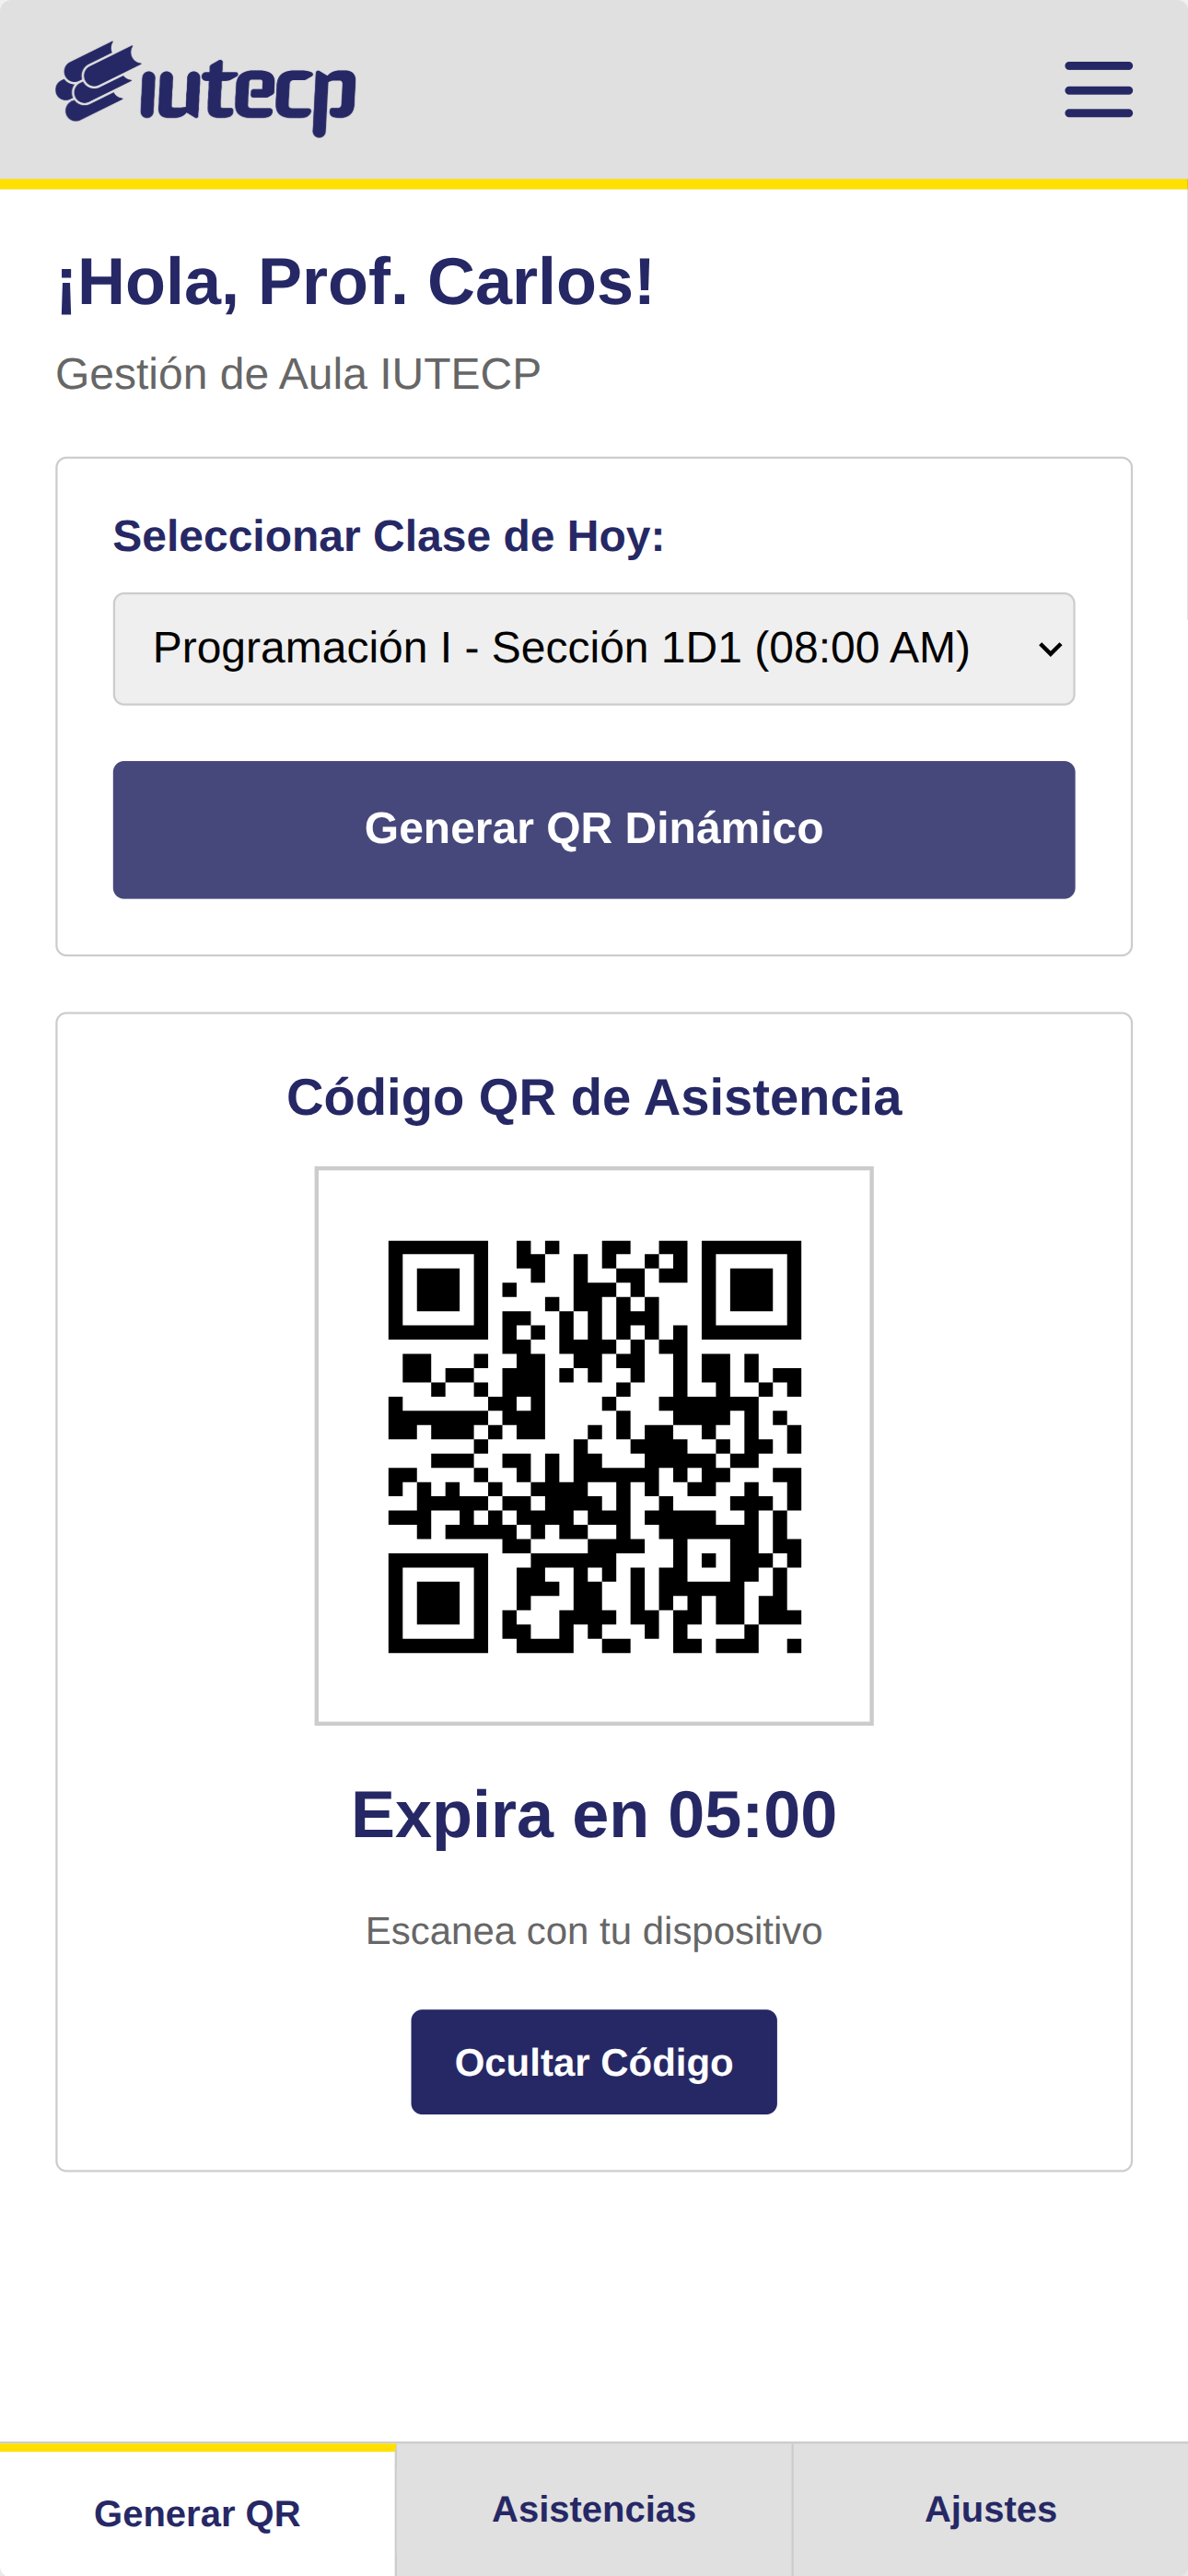
\includegraphics[width=0.3\textwidth]{../capturas/profegenerar_qr.png} &
  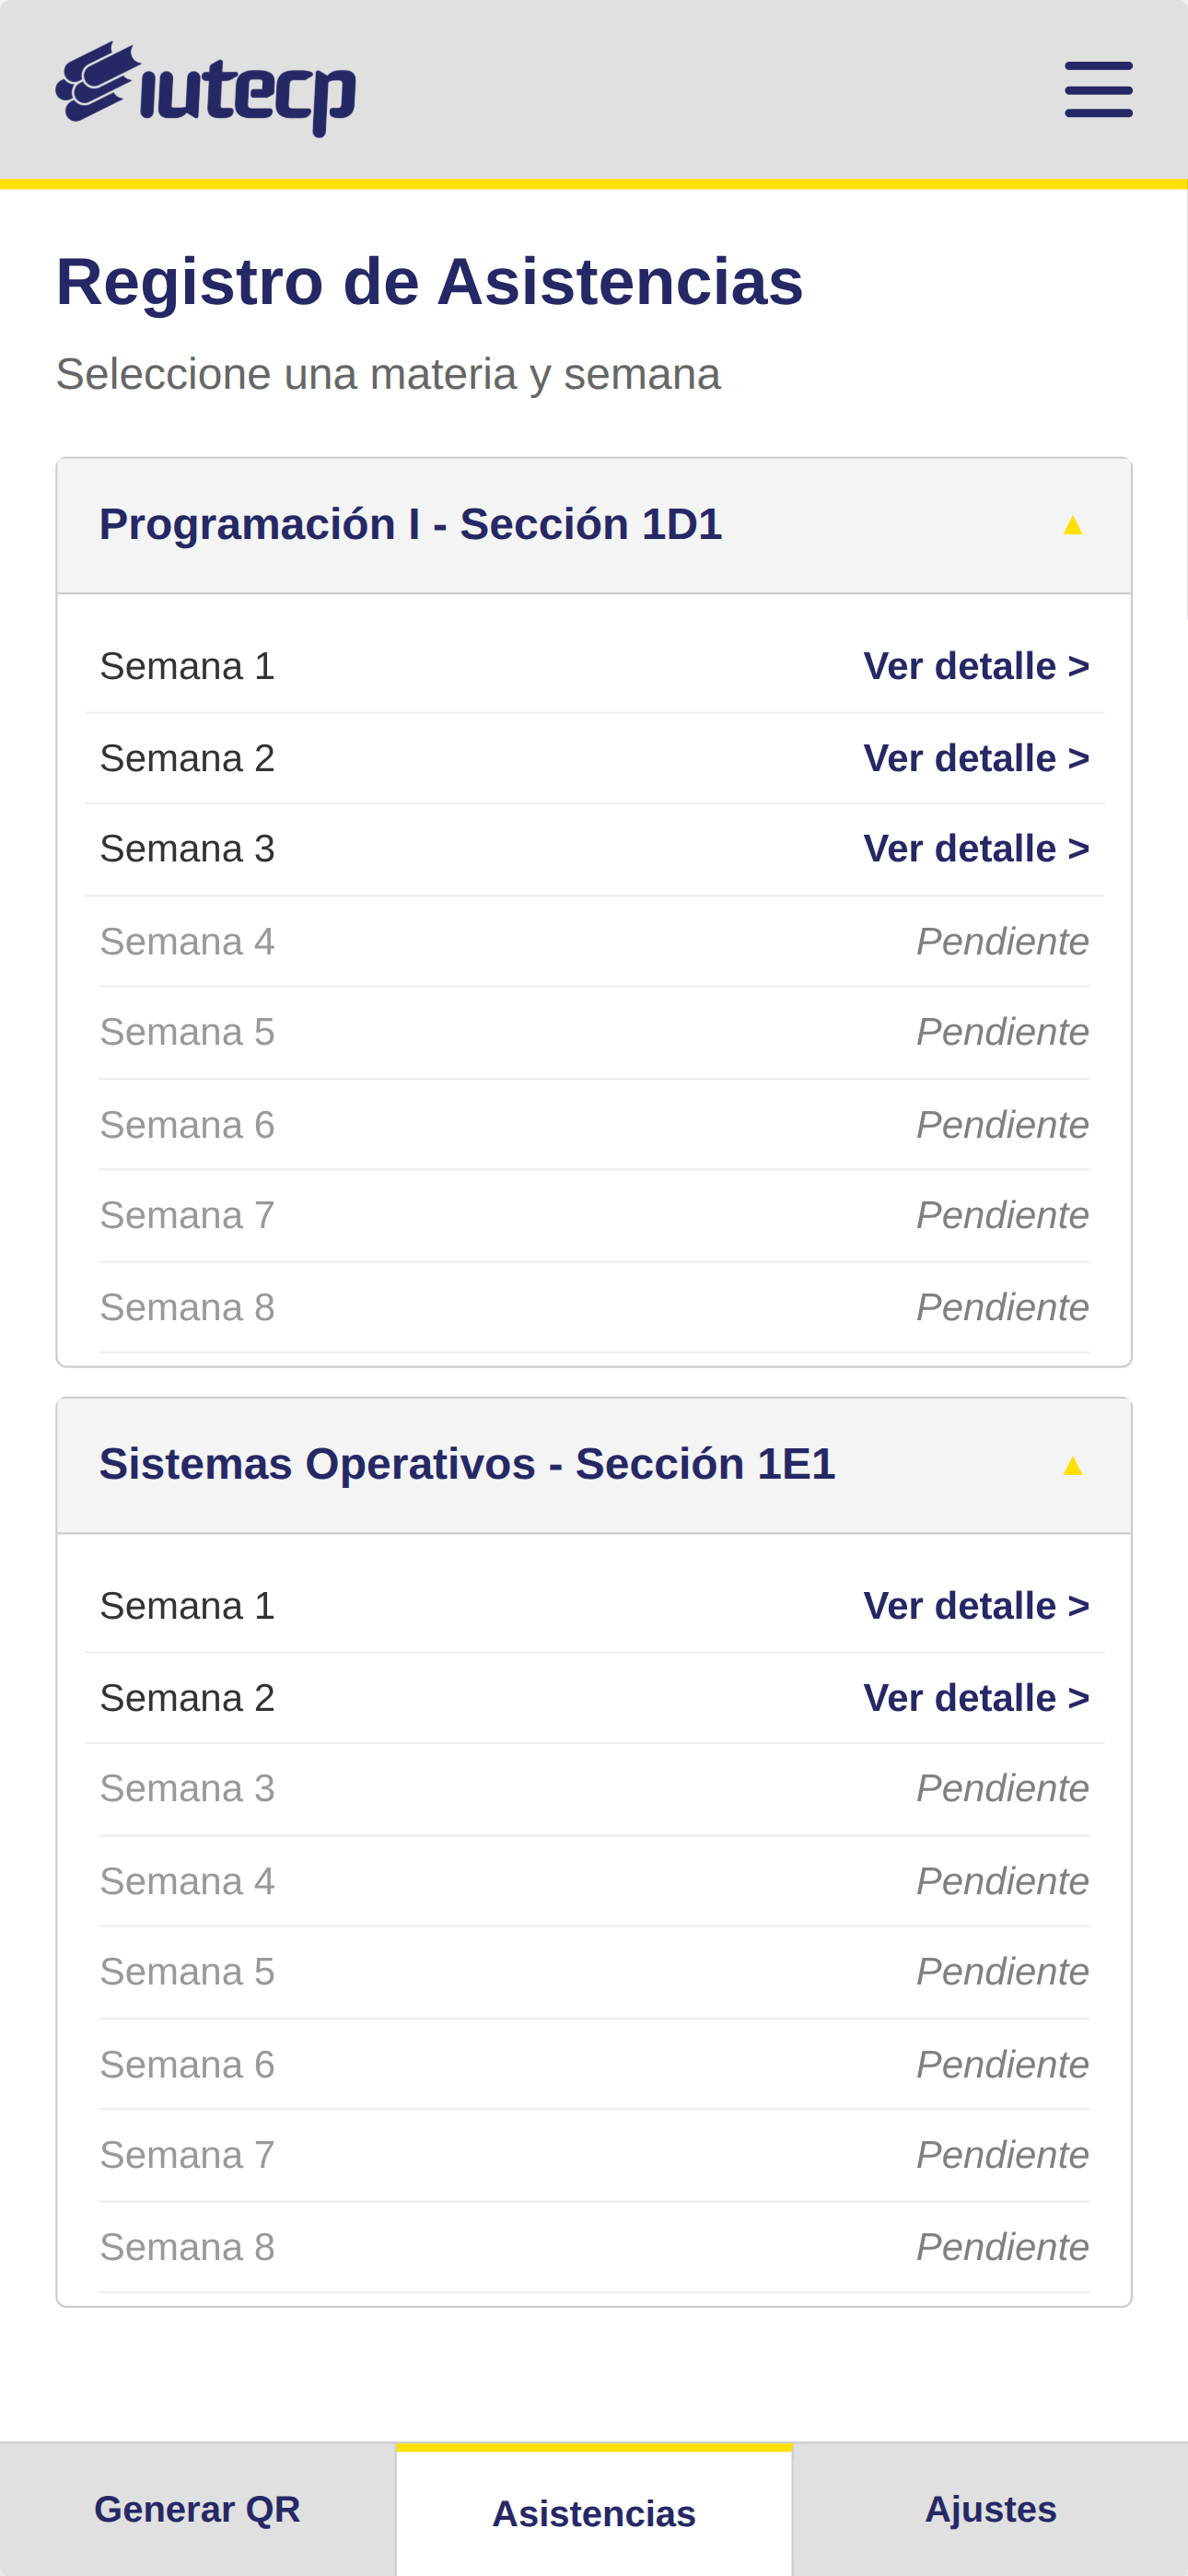
\includegraphics[width=0.3\textwidth]{../capturas/profeasistencias.png} &
  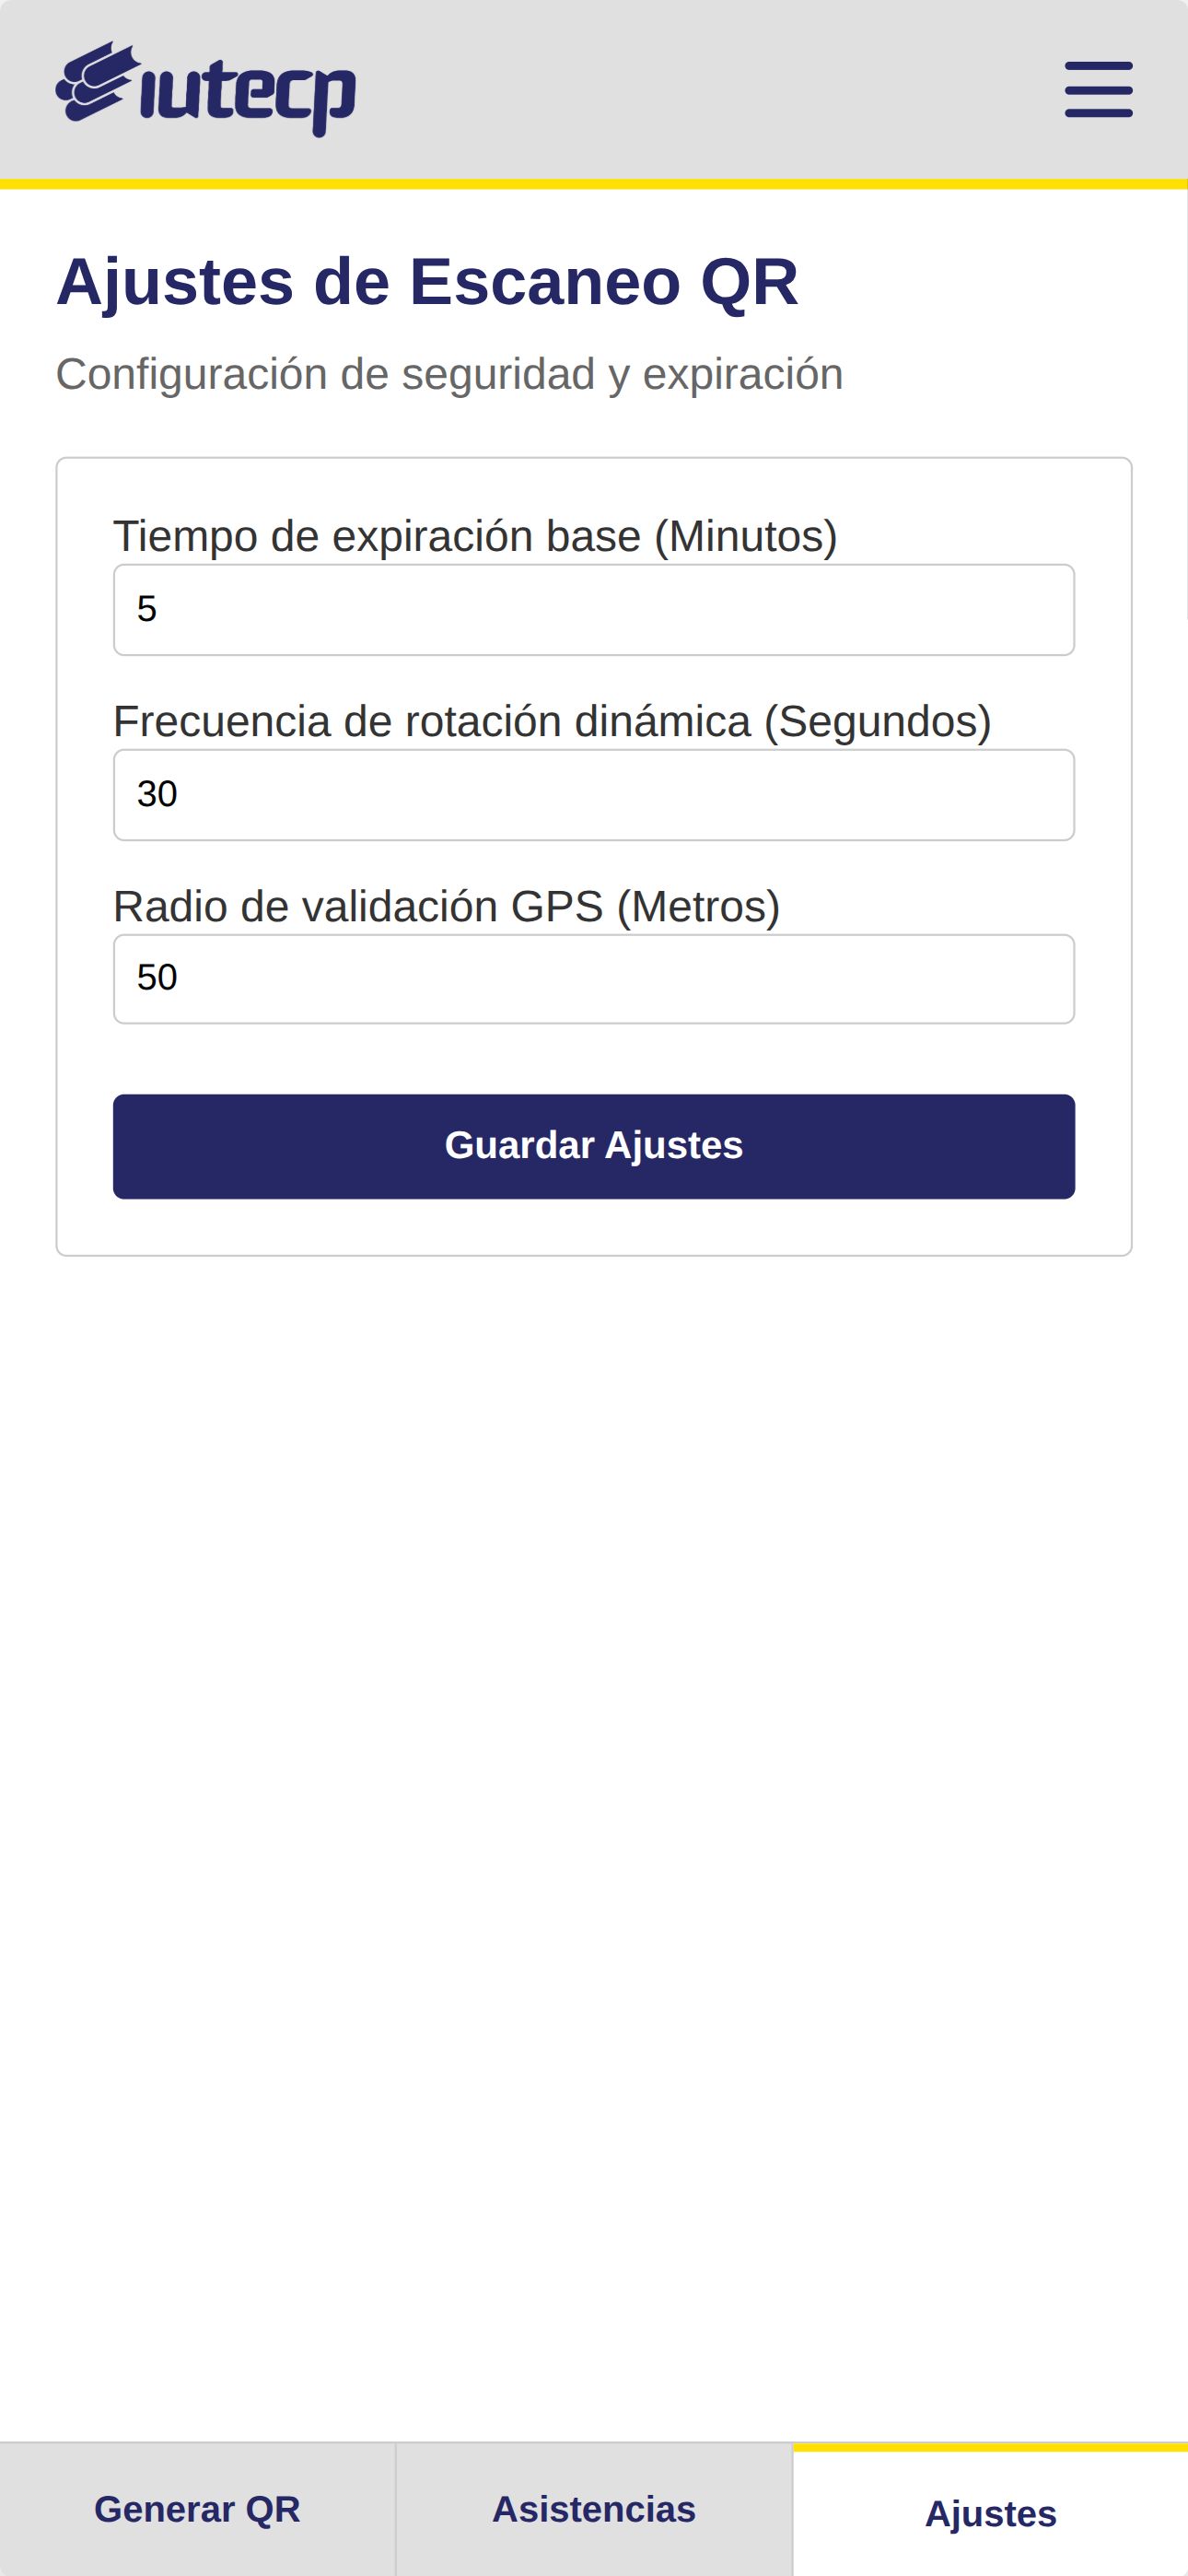
\includegraphics[width=0.3\textwidth]{../capturas/profeajustes.png} \\[2pt]
  \footnotesize\textbf{Profesor:} Generaci\'on QR &
  \footnotesize\textbf{Profesor:} Asistencias &
  \footnotesize\textbf{Profesor:} Ajustes \\[0.4cm]
  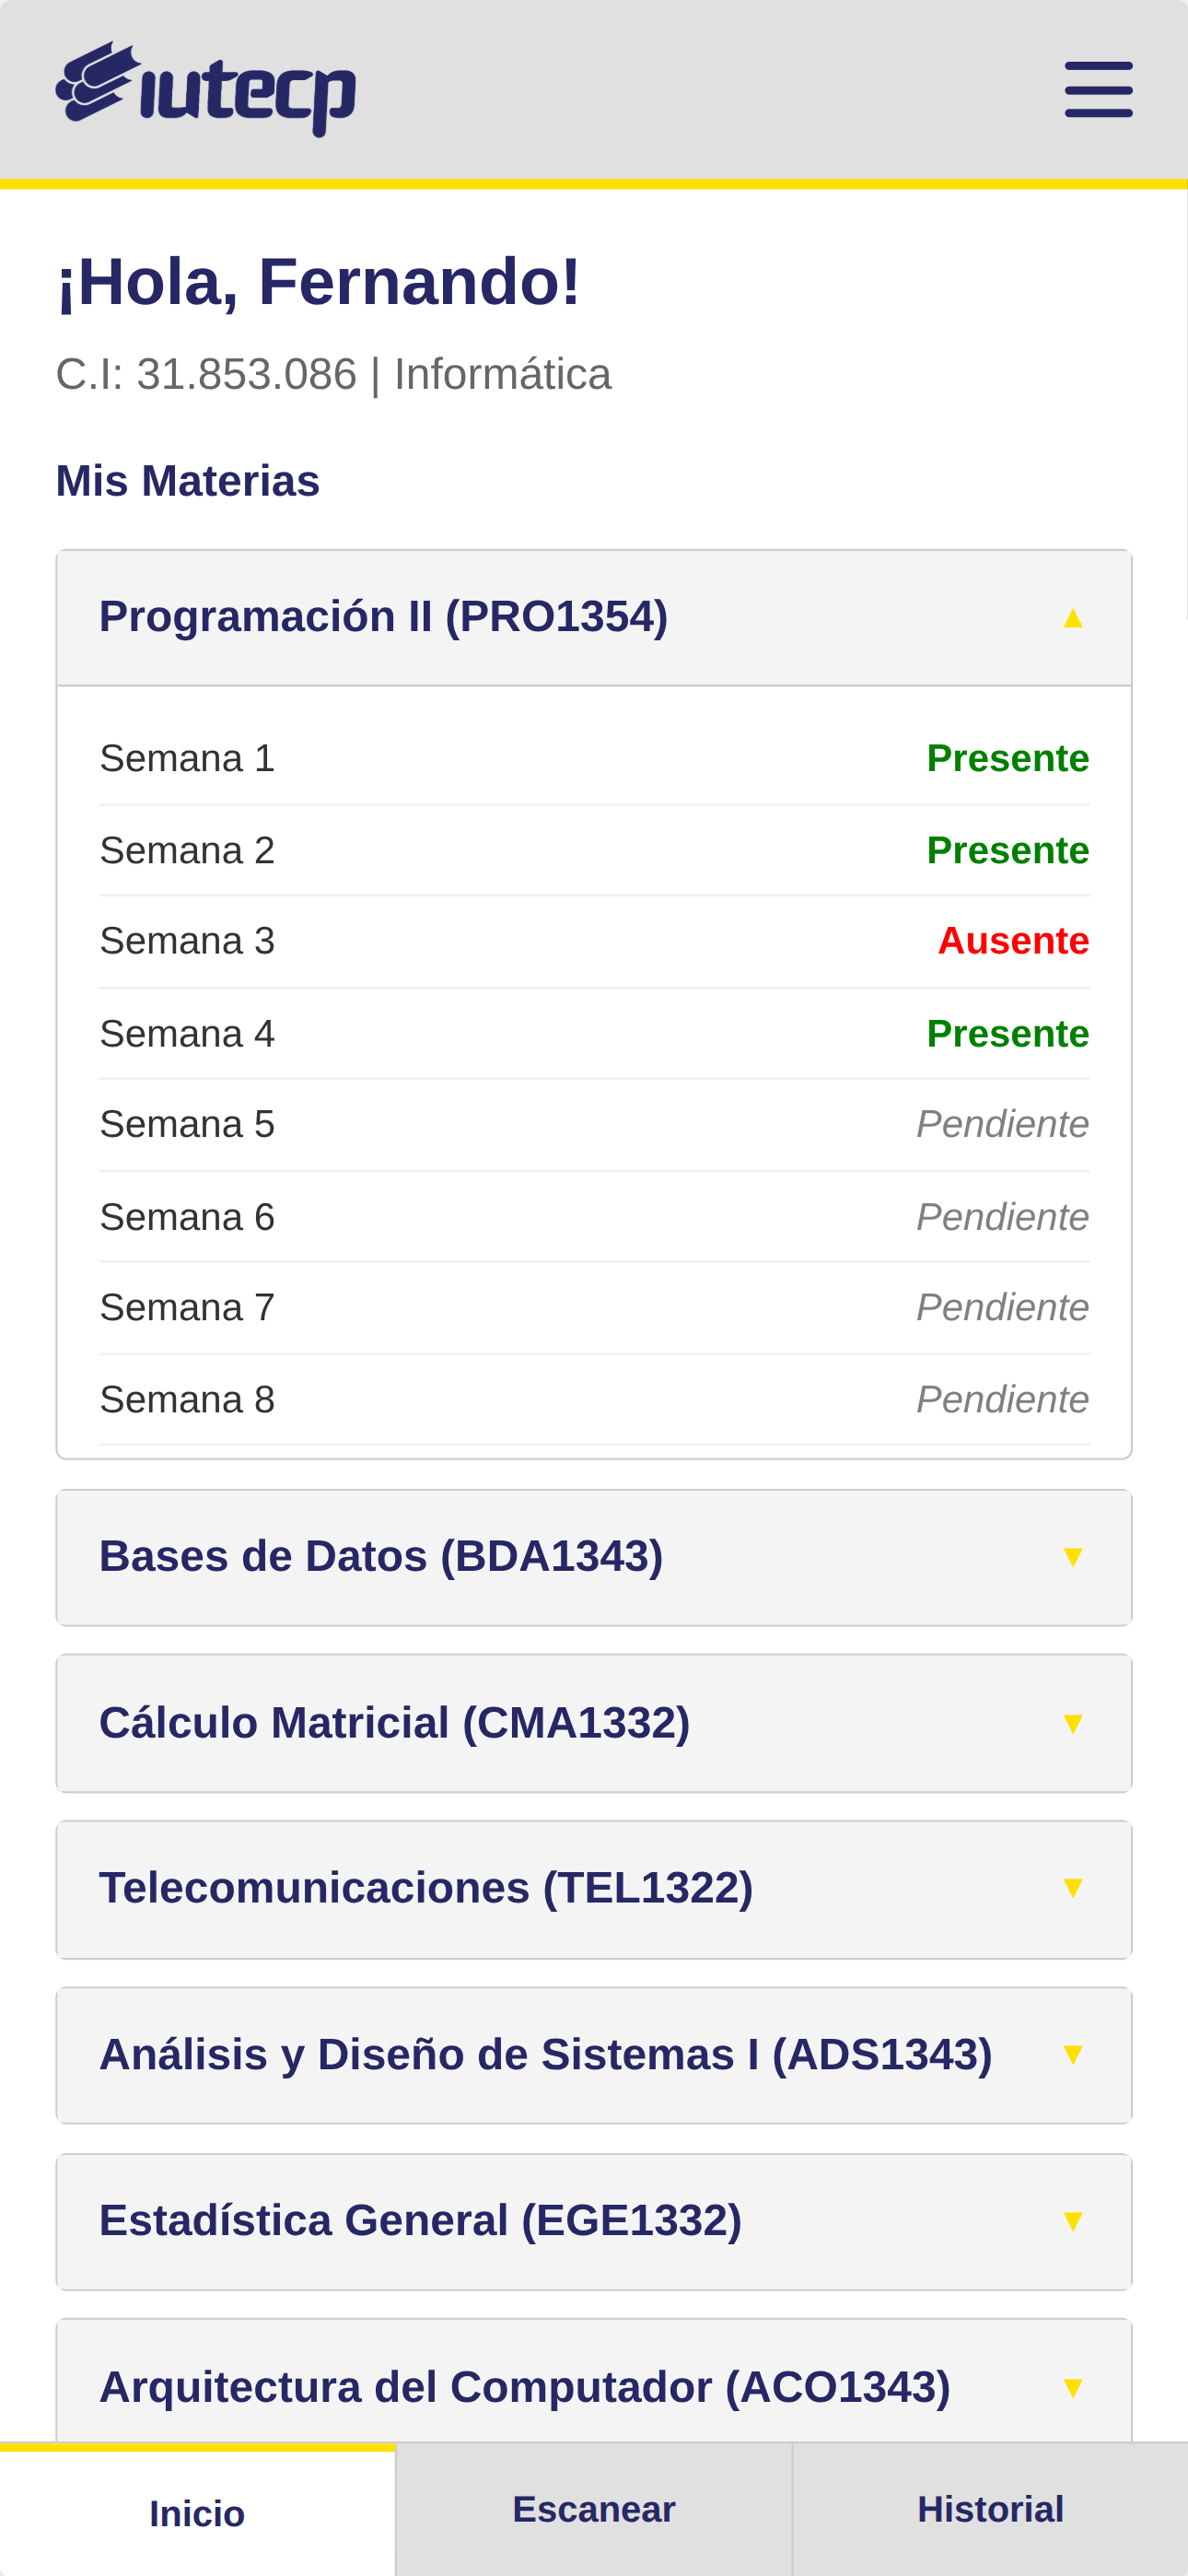
\includegraphics[width=0.3\textwidth]{../capturas/alumnoinicio.png} &
  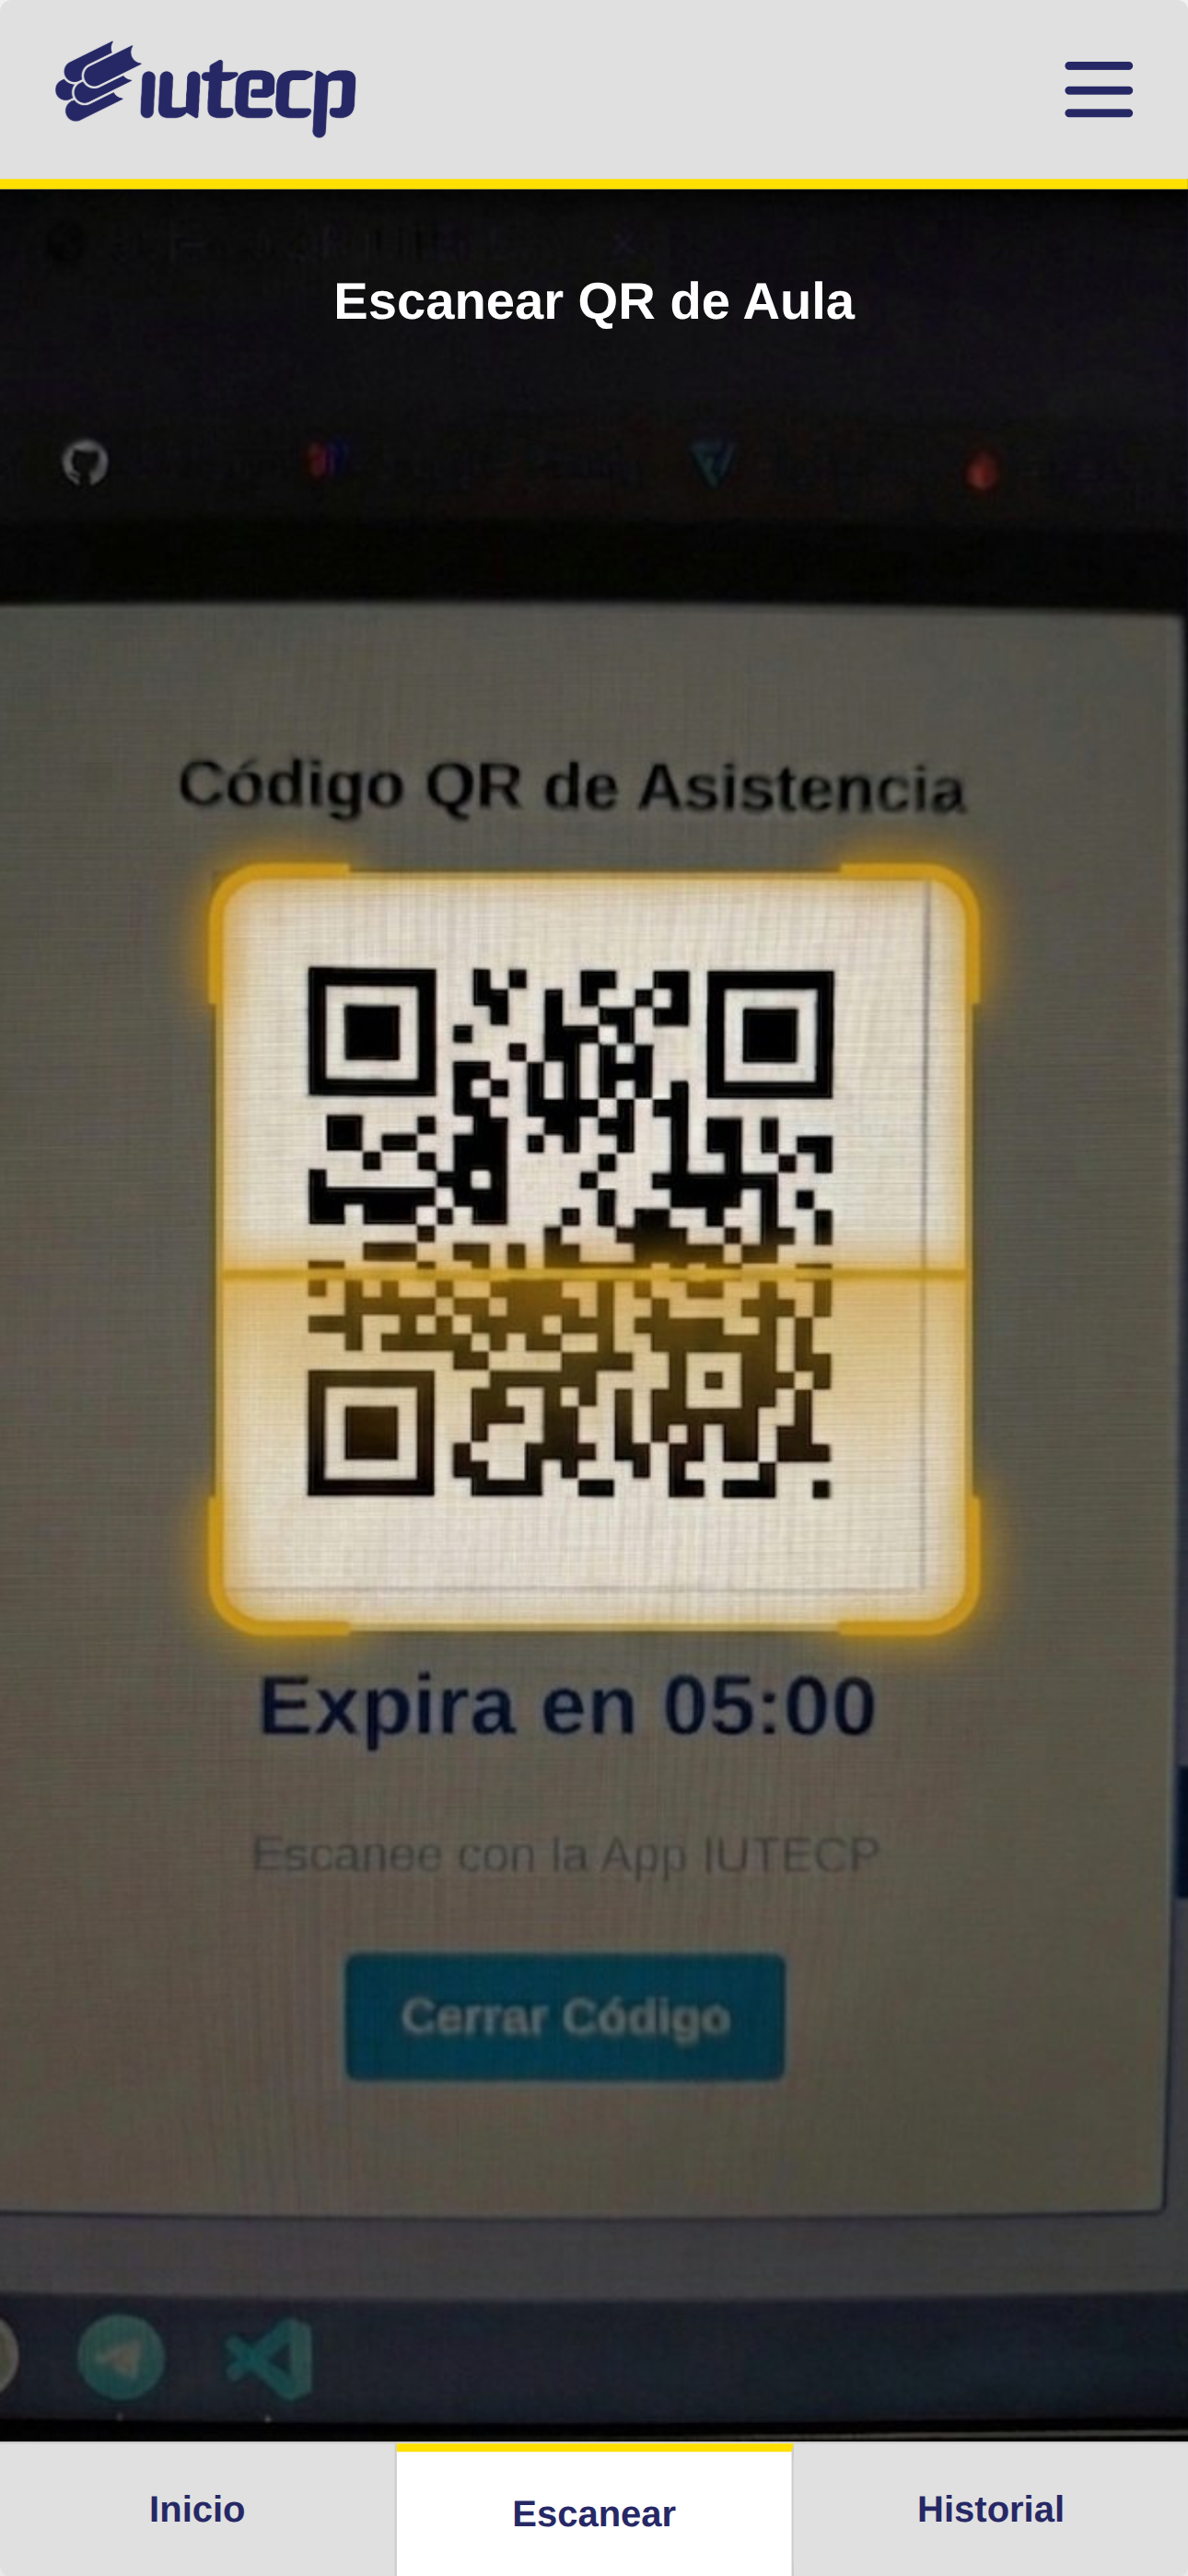
\includegraphics[width=0.3\textwidth]{../capturas/alumnoescaneo.png} &
  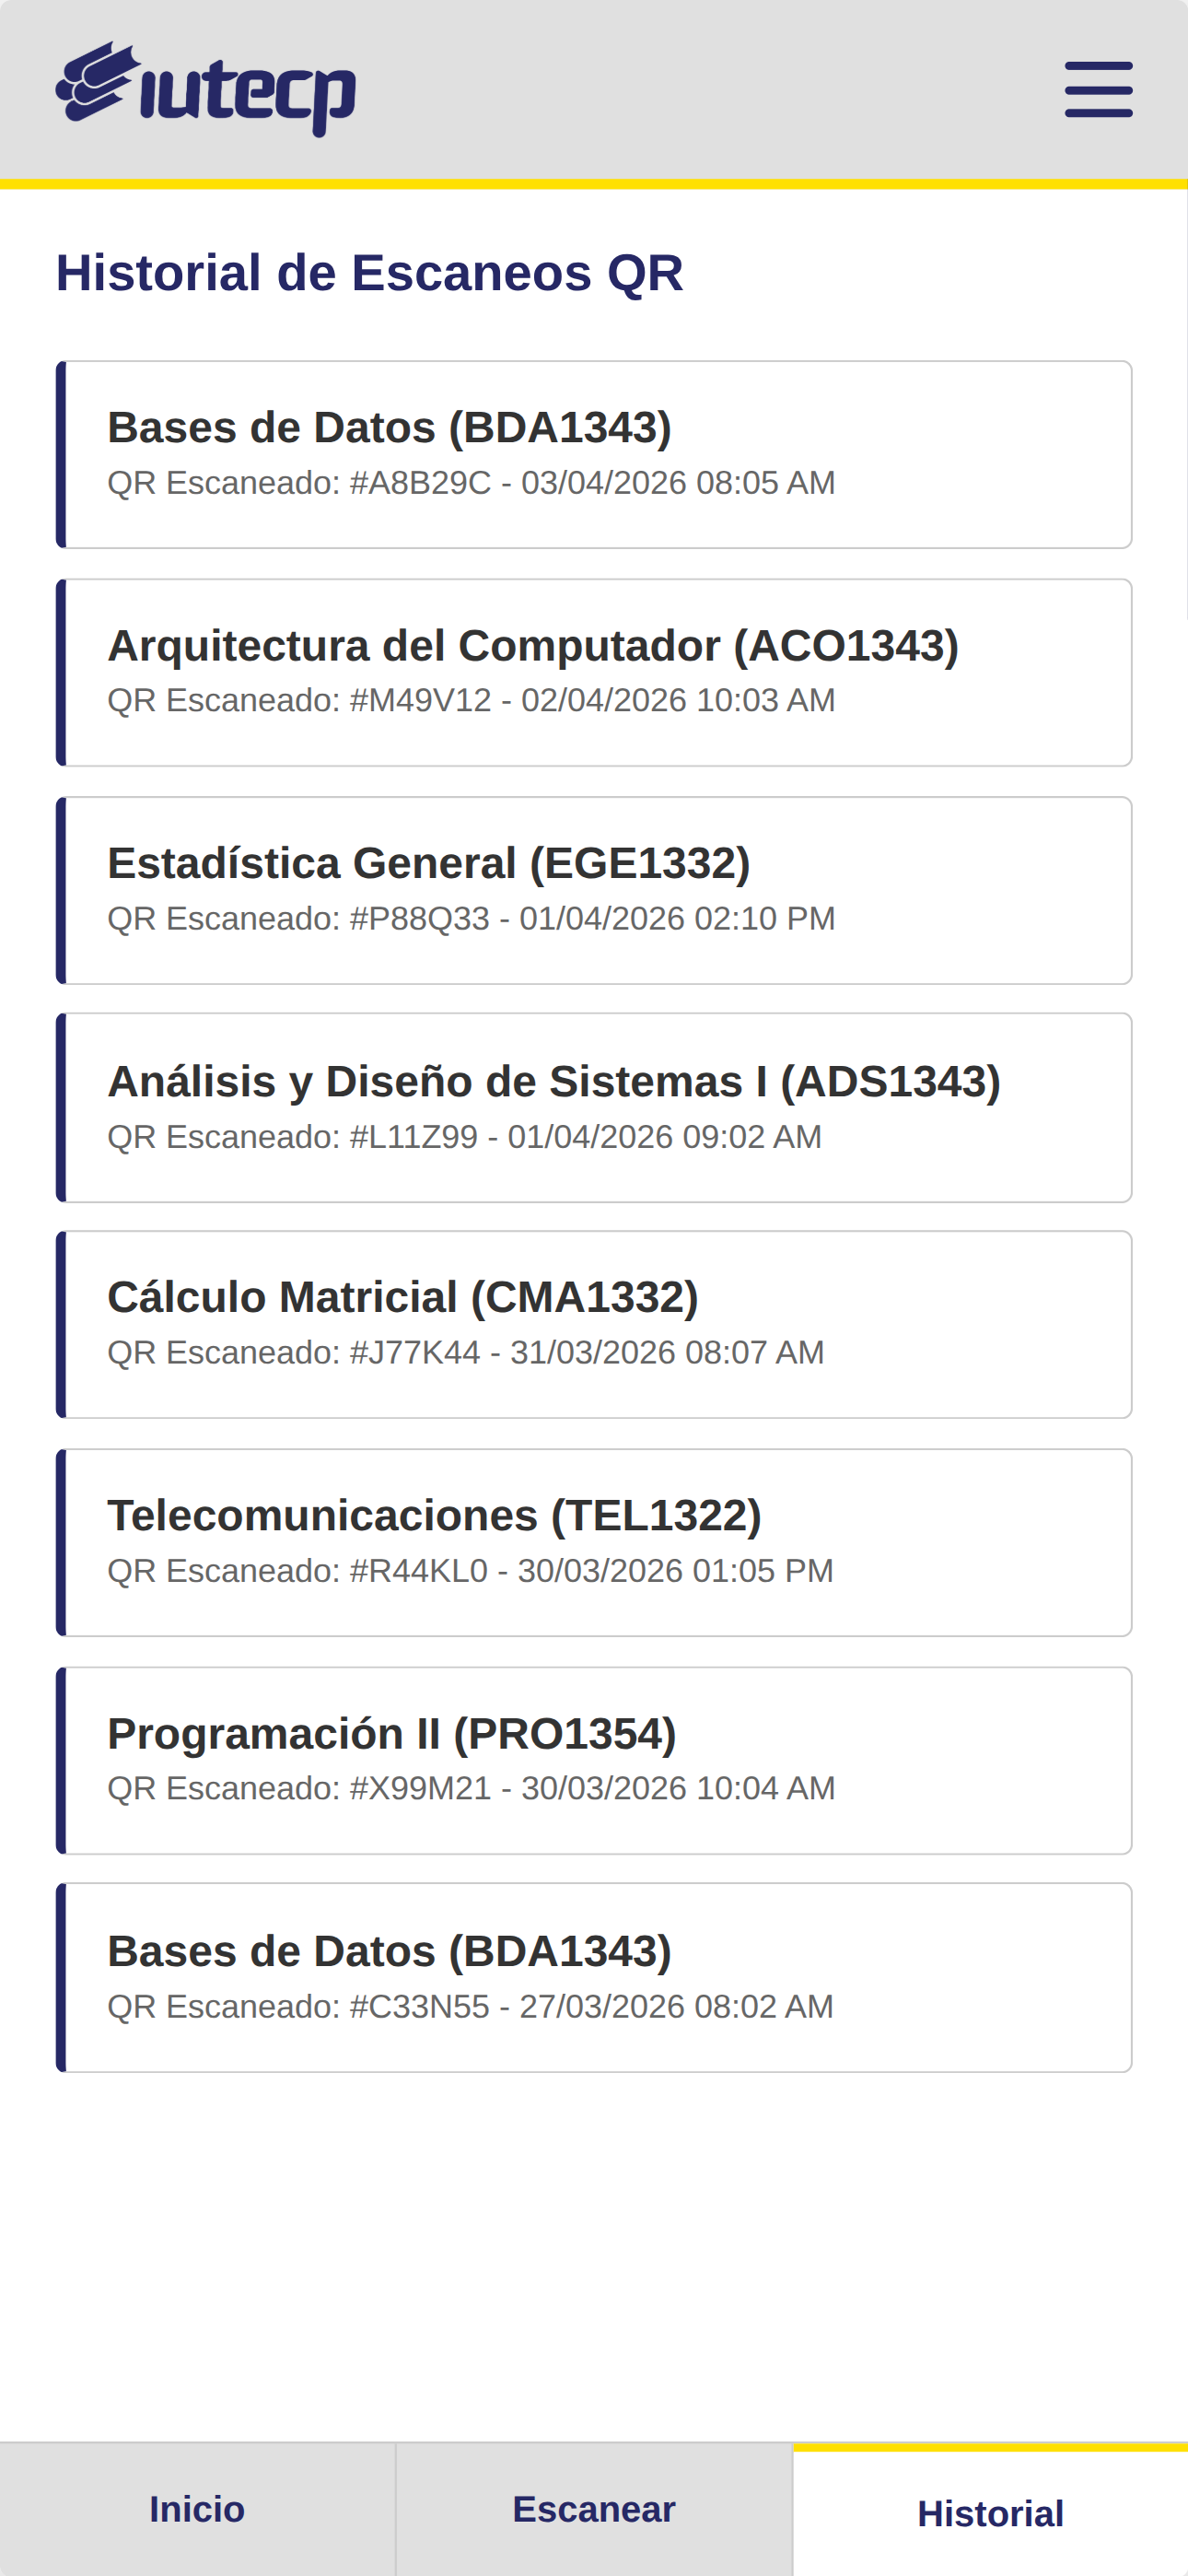
\includegraphics[width=0.3\textwidth]{../capturas/alumnohistorial.png} \\[2pt]
  \footnotesize\textbf{Estudiante:} Inicio &
  \footnotesize\textbf{Estudiante:} Escaneo QR &
  \footnotesize\textbf{Estudiante:} Historial
\end{tabular}
\end{center}

\newpage

\subsection*{Interfaces del Administrador}

Las siguientes capturas muestran las interfaces del panel de administrador, diseñadas en formato landscape para mejor visualización:

\begin{center}
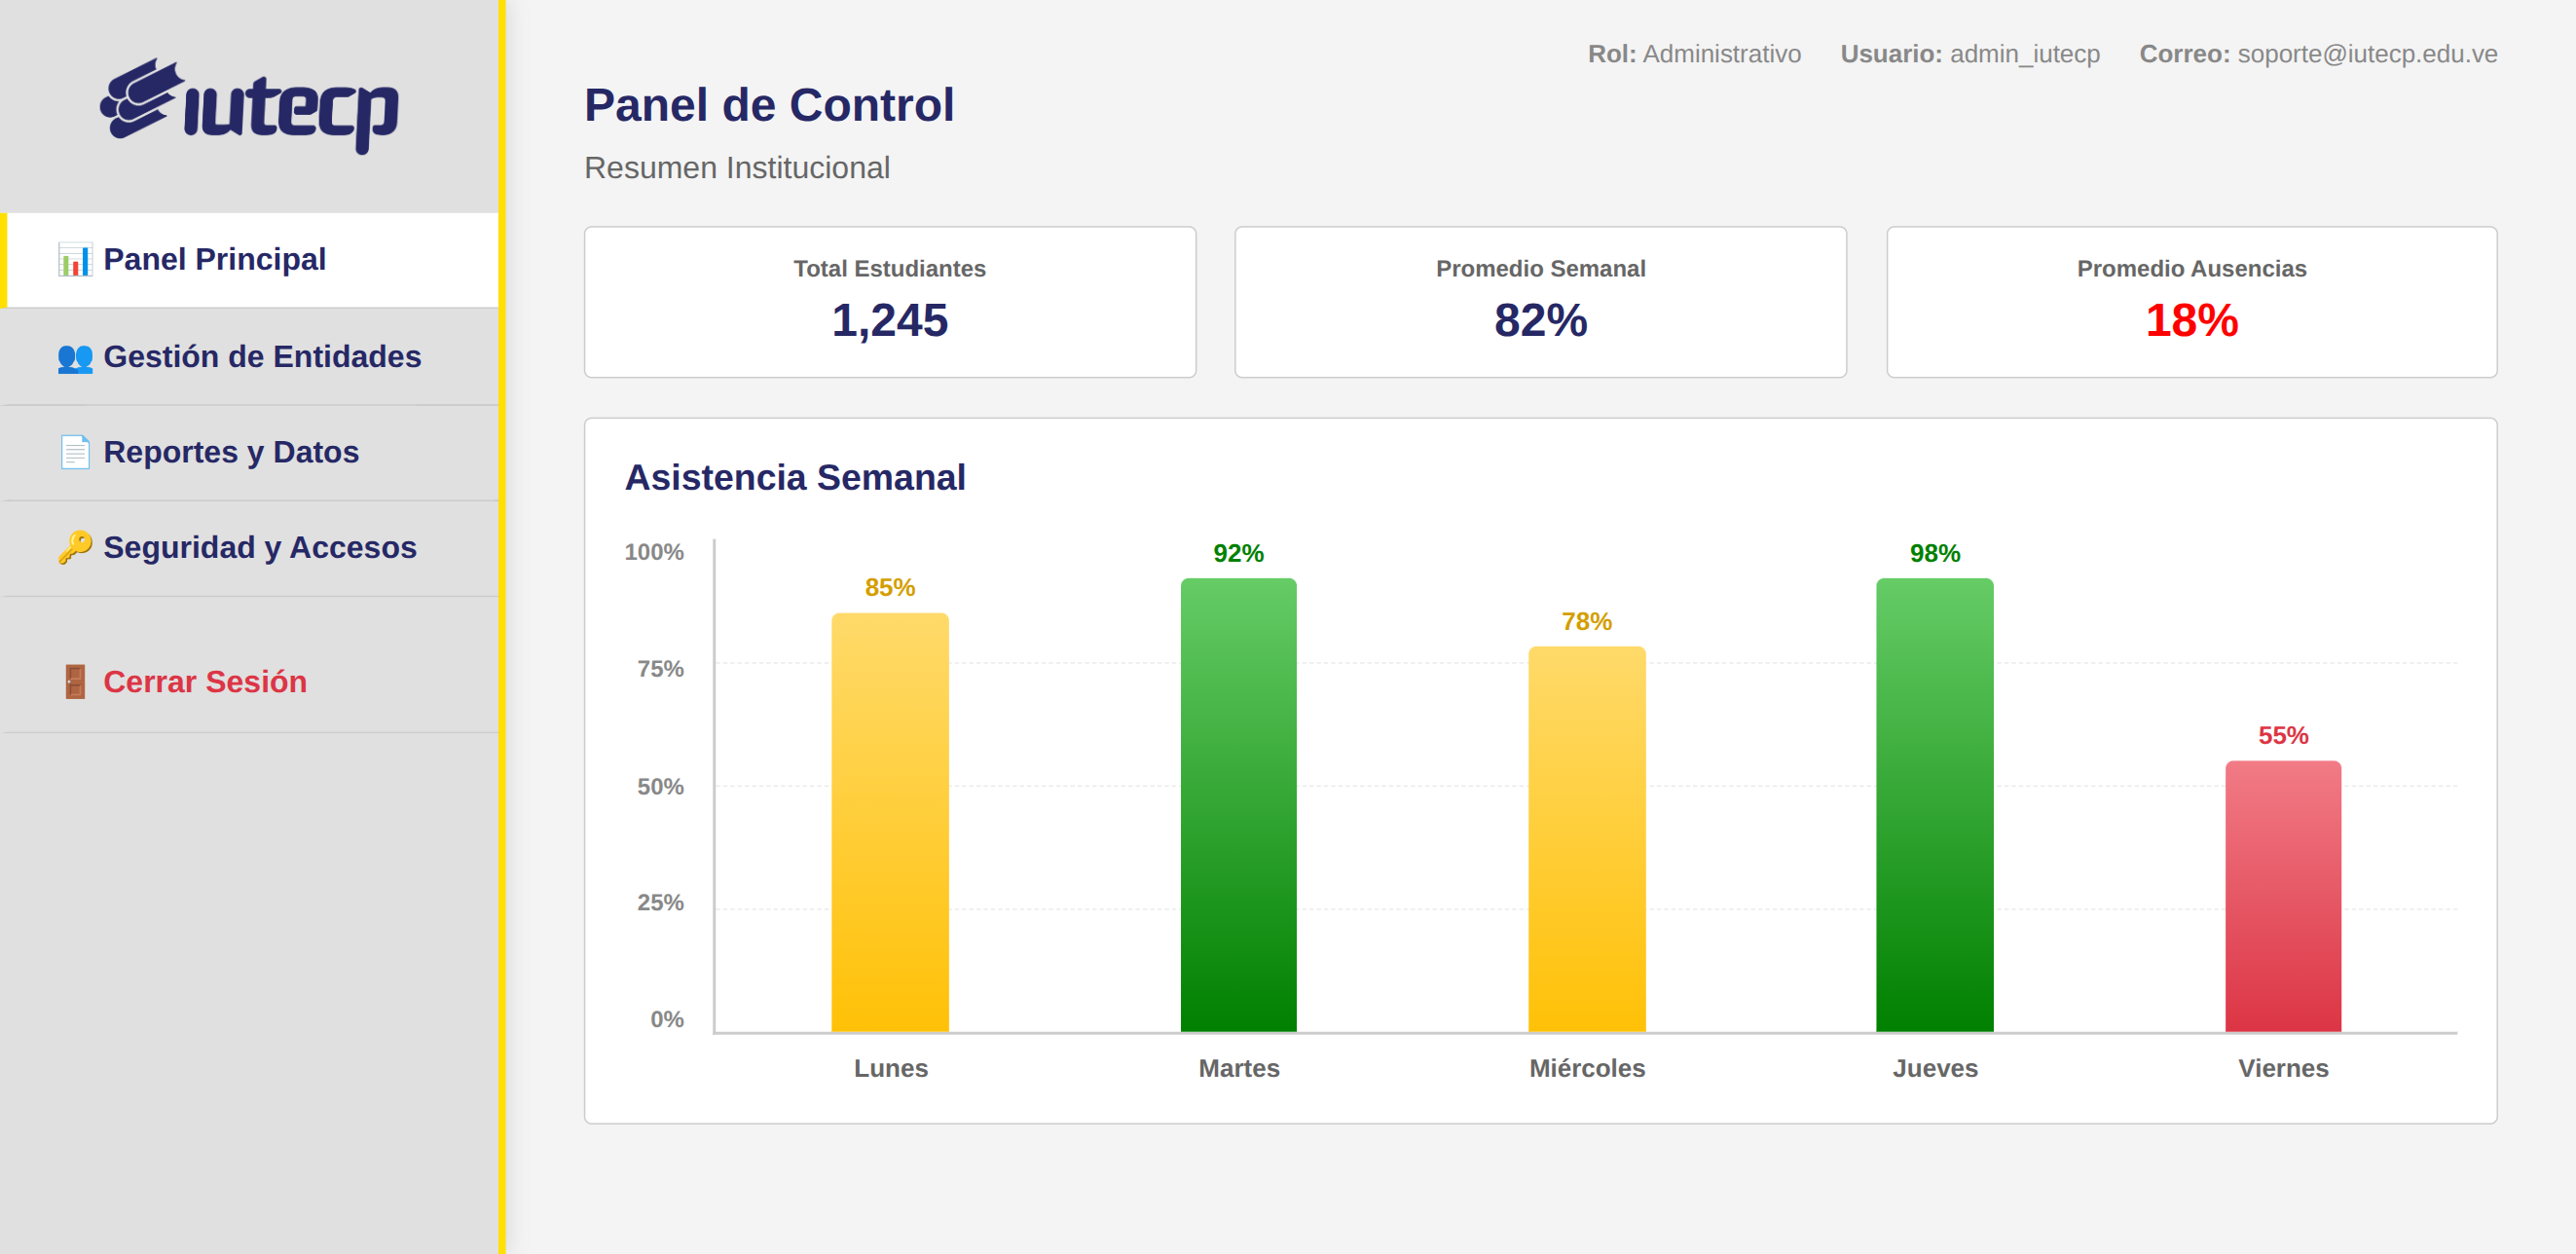
\includegraphics[width=0.8\textwidth]{../capturas/1panel_principal.png}

\vspace{0.2cm}

\textbf{Panel principal}

\vspace{0.3cm}

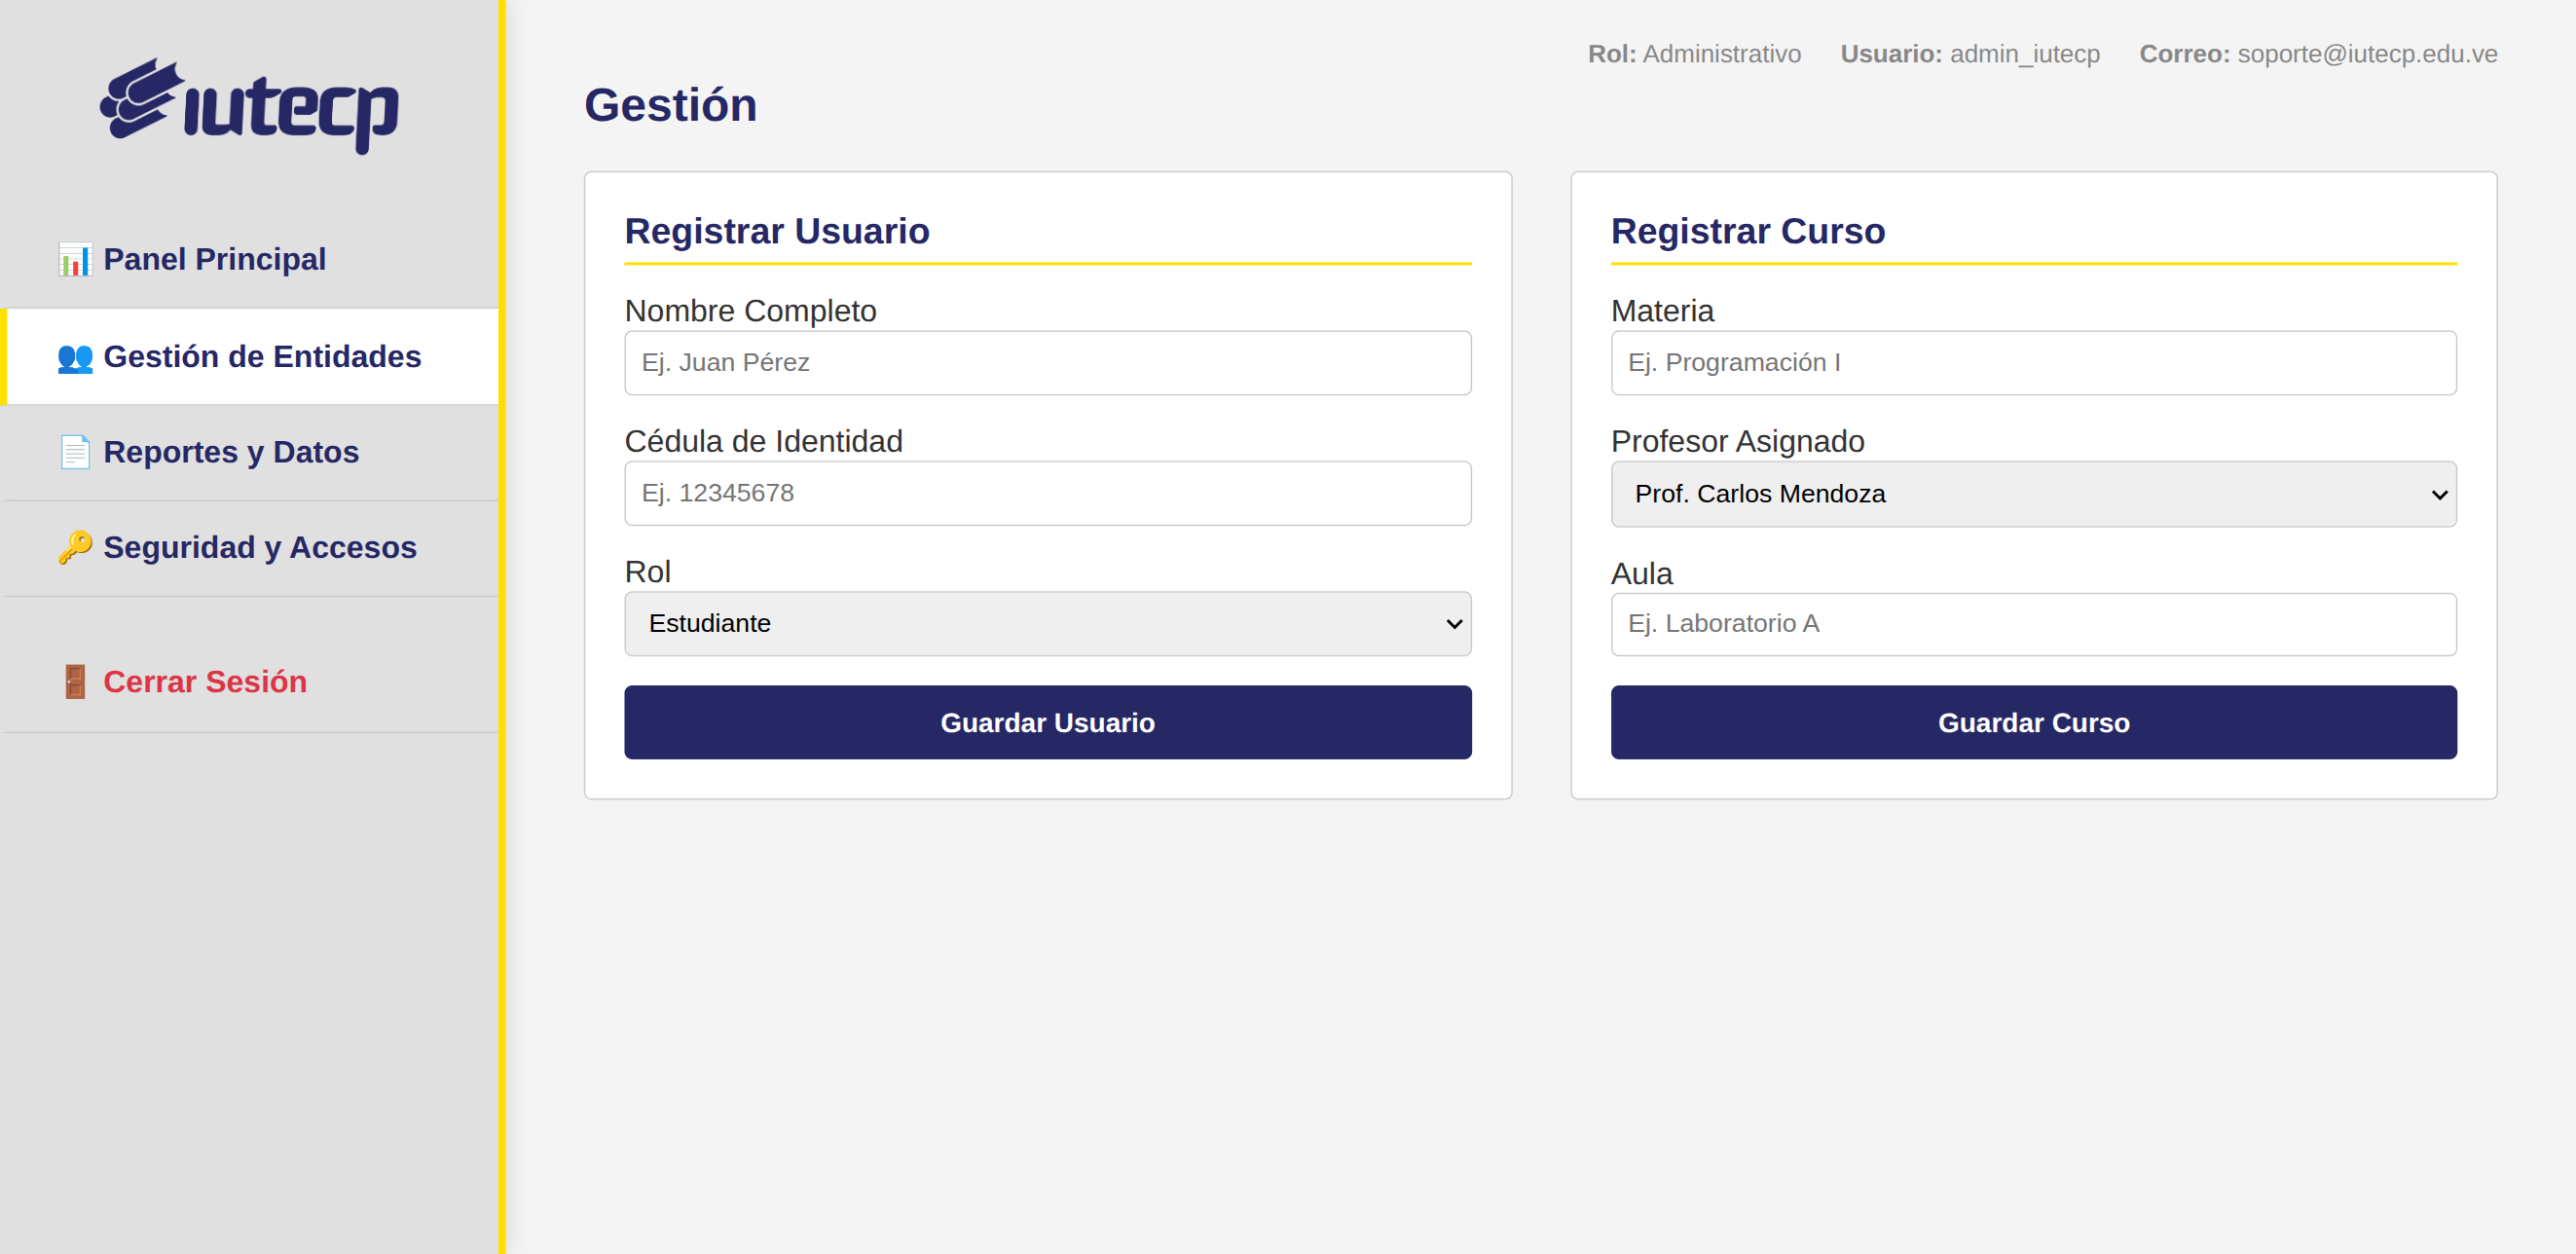
\includegraphics[width=0.8\textwidth]{../capturas/2gestion_de_entidades.png}

\vspace{0.2cm}

\textbf{Gestión de entidades}

\vspace{0.3cm}

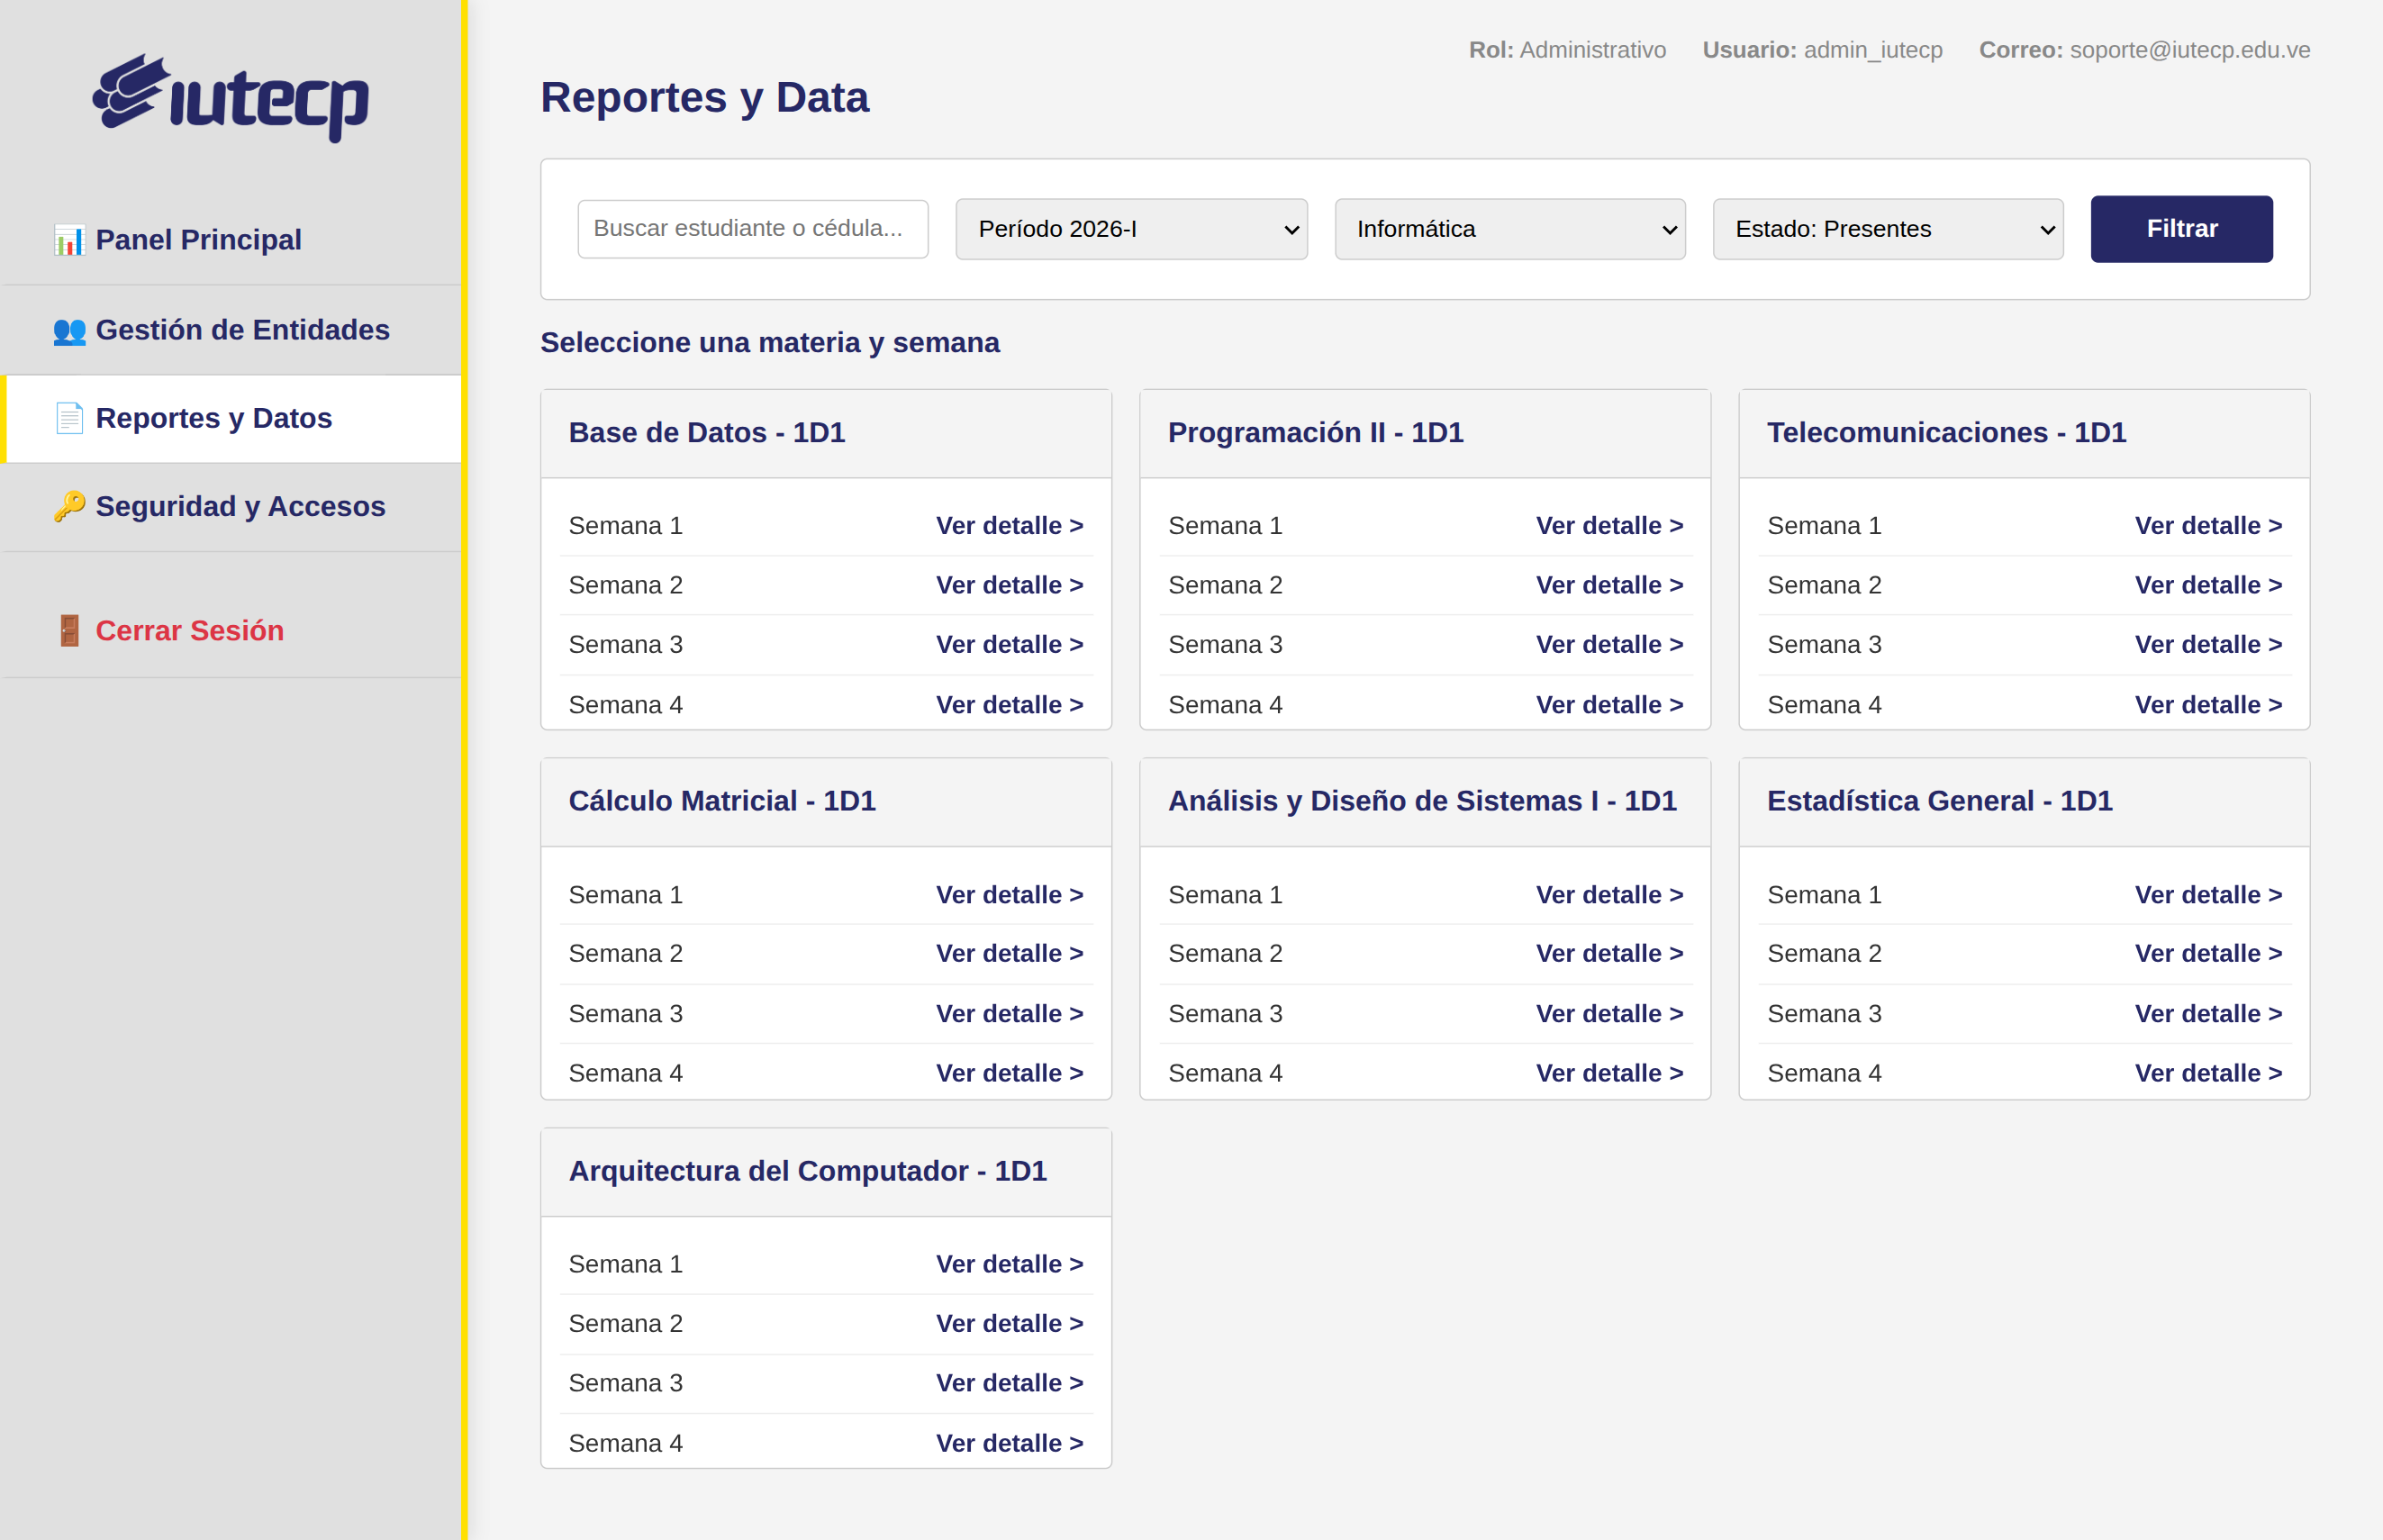
\includegraphics[width=0.8\textwidth]{../capturas/3reportes_y_datos.png}

\vspace{0.2cm}

\textbf{Reportes y datos}

\vspace{0.3cm}

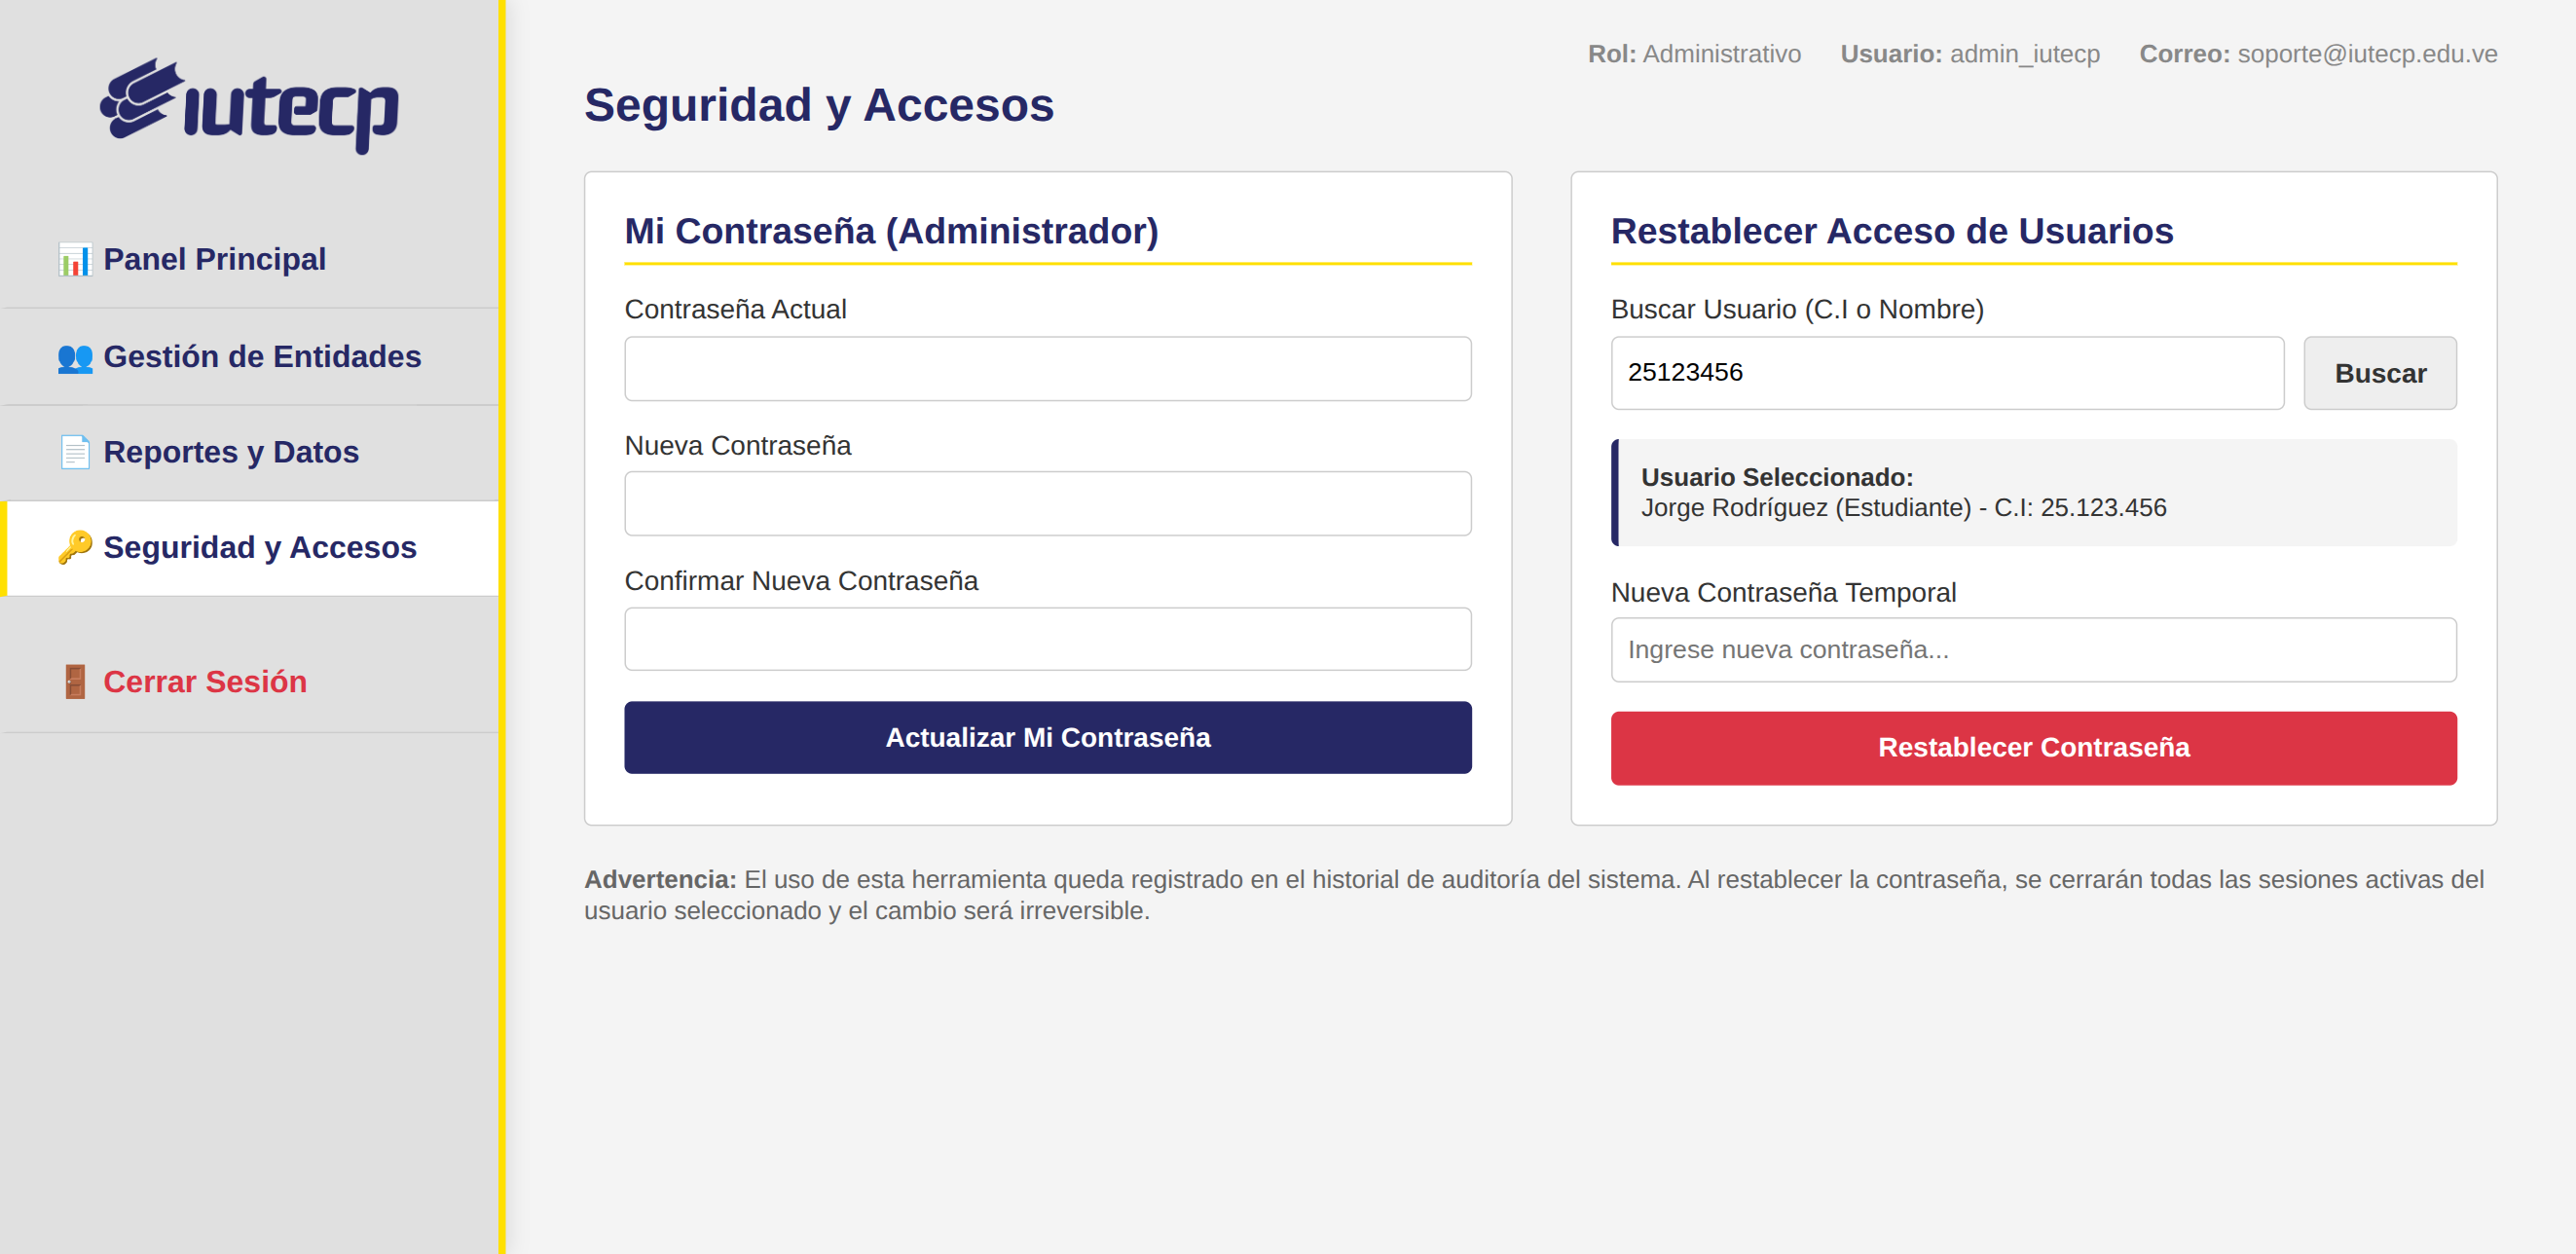
\includegraphics[width=0.8\textwidth]{../capturas/4seguridad_y_accesos.png}

\vspace{0.2cm}

\textbf{Seguridad y accesos}
\end{center}

\newpage

% ============================================================
% CAPÍTULO III
% ============================================================
\chapter{CREACI\'ON DE BASE DE DATOS Y\\LIBRER\'IAS DE PROGRAMAS}

\section{Base de Datos}

La base de datos del sistema, denominada \texttt{qr\_iutecp}, fue dise\~nada bajo el modelo relacional utilizando MariaDB 11.8 con motor InnoDB. Est\'a compuesta por trece tablas que en conjunto permiten gestionar usuarios, cursos, inscripciones, asistencias, sesiones QR, periodos acad\'emicos y auditor\'ia.

\subsection{Tablas del Sistema}

A continuaci\'on se describen las principales tablas que conforman la base de datos:

\begin{itemize}
  \item \texttt{usuarios:} Almacena los datos de todos los usuarios del sistema (administradores, profesores y estudiantes). Incluye campos como c\'edula (\'unico), nombre de usuario (\'unico), contrase\~na hasheada, correo electr\'onico, rol y estado (activo/inactivo).
  \item \texttt{carreras:} Contiene el cat\'alogo de carreras ofrecidas por la instituci\'on (Inform\'atica, Administraci\'on, Contadur\'ia).
  \item \texttt{cursos:} Registra las materias asociadas a cada carrera, con su c\'odigo, nombre, nivel, unidades cr\'edito y secci\'on.
  \item \texttt{inscripciones:} Relaciona estudiantes con los cursos en los que est\'an inscritos para un periodo acad\'emico espec\'ifico.
  \item \texttt{asistencias:} Registra el estado de asistencia (presente, ausente o justificado) de cada estudiante por semana y fecha, con restricci\'on de unicidad por inscripci\'on-semana-fecha.
  \item \texttt{sesiones\_qr:} Almacena los c\'odigos QR generados por los profesores, incluyendo el c\'odigo \'unico, la fecha de expiraci\'on, las coordenadas GPS y el radio permitido.
  \item \texttt{configuracion\_profesor:} Guarda la configuraci\'on personalizada de cada profesor: tiempo de expiraci\'on del QR, intervalo de rotaci\'on y radio GPS.
  \item \texttt{periodos:} Define los periodos acad\'emicos con sus fechas de inicio y fin, incluyendo soporte para estudiantes de nuevo ingreso.
  \item \texttt{auditoria:} Registra todas las acciones relevantes del sistema con identificador del usuario, tipo de acci\'on, descripci\'on, direcci\'on IP y marca de tiempo.
  \item \texttt{prerrequisitos:} Define las dependencias entre cursos para validar la disponibilidad de materias seg\'un el avance del estudiante.
\end{itemize}

\subsection{Esquema Relacional}

A continuaci\'on se presenta el script de creaci\'on de las tablas principales, ejecutado para generar la estructura de la base de datos:

\begin{lstlisting}[caption=Fragmento del esquema de base de datos (\texttt{sql/schema.sql})]
CREATE TABLE usuarios (
    id INT AUTO_INCREMENT PRIMARY KEY,
    cedula VARCHAR(20) NOT NULL UNIQUE,
    username VARCHAR(50) NOT NULL UNIQUE,
    password VARCHAR(255) NOT NULL,
    nombre VARCHAR(100) NOT NULL,
    email VARCHAR(100) NOT NULL,
    rol ENUM('admin', 'profesor', 'estudiante') NOT NULL,
    carrera_id INT,
    activo TINYINT(1) DEFAULT 1,
    password_temporal TINYINT(1) DEFAULT 1,
    FOREIGN KEY (carrera_id) REFERENCES carreras(id)
);

CREATE TABLE inscripciones (
    id INT AUTO_INCREMENT PRIMARY KEY,
    usuario_id INT NOT NULL,
    curso_id INT NOT NULL,
    periodo VARCHAR(10) NOT NULL,
    seccion VARCHAR(10),
    UNIQUE KEY (usuario_id, curso_id, periodo),
    FOREIGN KEY (usuario_id) REFERENCES usuarios(id),
    FOREIGN KEY (curso_id) REFERENCES cursos(id)
);

CREATE TABLE asistencias (
    id INT AUTO_INCREMENT PRIMARY KEY,
    inscripcion_id INT NOT NULL,
    semana INT NOT NULL,
    fecha DATE NOT NULL,
    estado ENUM('presente', 'ausente', 'justificado') DEFAULT 'ausente',
    UNIQUE KEY (inscripcion_id, semana, fecha),
    FOREIGN KEY (inscripcion_id) REFERENCES inscripciones(id)
);

CREATE TABLE sesiones_qr (
    id INT AUTO_INCREMENT PRIMARY KEY,
    profesor_id INT NOT NULL,
    curso_id INT NOT NULL,
    semana INT NOT NULL,
    codigo_qr VARCHAR(64) NOT NULL UNIQUE,
    expira_en DATETIME NOT NULL,
    FOREIGN KEY (profesor_id) REFERENCES usuarios(id),
    FOREIGN KEY (curso_id) REFERENCES cursos(id)
);
\end{lstlisting}

\section{Librer\'ias de Programas}

El sistema organiza su c\'odigo en librer\'ias reutilizables ubicadas en el directorio \texttt{includes/}, las cuales centralizan la l\'ogica com\'un yevitan la duplicaci\'on de c\'odigo. A continuaci\'on se describen las principales:

% Subsecciones NO numeradas para que no aparezcan en la TOC
\subsection*{Configuraci\'on y Conexi\'on (\texttt{config.php})}

Este archivo establece la conexi\'on a la base de datos mediante PDO (\textit{PHP Data Objects}), configurando el manejo de errores en modo excepci\'on y el juego de caracteres UTF-8. La conexi\'on se almacena en la variable \$pdo, utilizada por todos los m\'odulos del sistema.

\subsection*{Manejo de Sesiones (\texttt{session.php})}

Contiene las funciones de autenticaci\'on y control de acceso:
\begin{itemize}
  \item \texttt{estaAutenticado():} Verifica si el usuario ha iniciado sesi\'on.
  \item \texttt{redirigirSegunRol():} Redirige al usuario al panel correspondiente seg\'un su rol.
  \item \texttt{registrarAuditoria():} Inserta registros en la tabla de auditor\'ia para rastrear las acciones de los usuarios.
\end{itemize}

\subsection*{Funciones Utilitarias (\texttt{functions.php})}

Agrupa funciones de uso general:
\begin{itemize}
  \item \texttt{generarPasswordTemporal():} Genera contrase\~nas aleatorias seguras para nuevos usuarios.
  \item \texttt{limpiarInput():} Sanitiza datos de entrada para prevenir XSS.
  \item \texttt{generarUsername():} Crea nombres de usuario autom\'aticos basados en el nombre y apellido.
\end{itemize}

\subsection*{L\'ogica Acad\'emica (\texttt{academico.php})}

Implementa la l\'ogica relacionada con la gesti\'on acad\'emica:
\begin{itemize}
  \item \texttt{obtenerPeriodoActivo():} Determina el periodo acad\'emico vigente.
  \item \texttt{obtenerSemanaActual():} Calcula la semana acad\'emica actual seg\'un la fecha de inicio del periodo.
  \item \texttt{verificarPrerrequisitos():} Valida si un estudiante cumple con los prerrequisitos necesarios para cursar una materia.
  \item \texttt{obtenerMateriasDisponibles():} Retorna las materias que un estudiante puede cursar seg\'un su avance en el pensum.
\end{itemize}

\subsection*{Generaci\'on de C\'odigos QR (\texttt{phpqrcode/phpqrcode.php})}

Se utiliza la biblioteca \textit{PHP QR Code} (versi\'on 1.1.4) para la generaci\'on de c\'odigos QR. Esta librer\'ia, bajo licencia LGPL 3, proporciona funciones para crear c\'odigos QR a partir de texto, URLs o datos estructurados. El archivo incluido es una versi\'on fusionada que no requiere archivos externos y viene configurada con caché deshabilitada y una b\'usqueda de m\'as rápida. El sistema emplea esta biblioteca para generar c\'odigos QR \'unicosen para cada sesi\'on de clase, con expiraci\'on configurable y soporte para geolocalizaci\'on.

\newpage

% ============================================================
% REFERENCIAS
% ============================================================
\pagestyle{body}
\begin{singlespace}

\section*{REFERENCIAS}
\addcontentsline{toc}{chapter}{REFERENCIAS}

\begin{enumerate}
\item PHP Group. (2024). \textit{PHP Manual}. \url{https://www.php.net/manual}
\item MariaDB Foundation. (2024). \textit{MariaDB Knowledge Base}. \url{https://mariadb.com/kb}
\item Pressman, R. S. (2014). \textit{Ingenier\'ia del software: Un enfoque pr\'actico} (7.a ed.). McGraw-Hill.
\item Sommerville, I. (2011). \textit{Ingenier\'ia de software} (9.a ed.). Pearson.
\item W3C. (2023). \textit{HTML Living Standard}. \url{https://html.spec.whatwg.org}
\item MDN Web Docs. (2024). \textit{JavaScript Guide}. \url{https://developer.mozilla.org}
\item Dominik Dzienia. (2010). \textit{PHP QR Code Encoder}. \url{http://phpqrcode.sourceforge.net}
\end{enumerate}

\end{singlespace}

\end{document}